\documentclass[a4paper,12pt]{article}

% General document formatting
%\usepackage[margin=0.7in]{geometry}
\usepackage[parfill]{parskip}
\usepackage{url, hyperref}
\usepackage{color}
\usepackage[usestackEOL]{stackengine}[2013-10-15] % formatting Pascal
\usepackage[dvipsnames]{xcolor}

\usepackage{cancel}
\usepackage[export]{adjustbox}

% Related to math
\usepackage{amsmath,amssymb,amsfonts,amsthm}
\usepackage{mathtools}
\usepackage{tikz}
\DeclarePairedDelimiter\norm{\lVert}{\rVert}
\newcommand{\innerproduct}[2]{\langle #1, #2 \rangle}
\usepackage{algorithm}
\usepackage{algpseudocode}

% encoding and language
\usepackage{lmodern}
\usepackage[slovene]{babel}
\usepackage[utf8]{inputenc}
\usepackage[T1]{fontenc}
\usepackage[mathscr]{euscript}

% multiline comments
\usepackage{verbatim}

% images
\usepackage{graphicx}
\graphicspath{ {./images/} }

% tags
\usepackage{pifont}
% \tag{\ding{37}} - telefon

% theorems
\theoremstyle{definition}
\newtheorem{counter}{Counter}[section] % not for use
\newtheorem{defn}[counter]{Definicija}
\newtheorem{lemma}[counter]{Lema}
\newtheorem{conseq}[counter]{Posledica}
\newtheorem{claim}[counter]{Trditev}
\newtheorem{theorem}[counter]{Izrek}
%%
\theoremstyle{remark}
\newtheorem*{ex}{Primer}
\newtheorem*{rem}{Opomba}
\newtheorem{rem*}[counter]{Opomba}
\newtheorem{ex*}[counter]{Primer}

% I like my squares DARK
\renewcommand\qedsymbol{$\blacksquare$}

% common commands redefined convenience purposes
\newcommand{\N}{\mathbb{N}}
\newcommand{\Z}{\mathbb{Z}}
\newcommand{\Q}{\mathbb{Q}}
\newcommand{\R}{\mathbb{R}}
\newcommand{\C}{\mathbb{C}}
\newcommand{\Pp}{\mathbb{P}}
\newcommand{\ch}{\operatorname{char}}

% subsubsubsections (paragraphs)
\usepackage{titlesec}
\usepackage{hyperref}

\titleclass{\subsubsubsection}{straight}[\subsection]

\newcounter{subsubsubsection}[subsubsection]
\renewcommand\thesubsubsubsection{\thesubsubsection.\arabic{subsubsubsection}}
\renewcommand\theparagraph{\thesubsubsubsection.\arabic{paragraph}} % optional; useful if paragraphs are to be numbered

\titleformat{\subsubsubsection}
  {\normalfont\normalsize\bfseries}{\thesubsubsubsection}{1em}{}
\titlespacing*{\subsubsubsection}
{0pt}{3.25ex plus 1ex minus .2ex}{1.5ex plus .2ex}

\makeatletter
\renewcommand\paragraph{\@startsection{paragraph}{5}{\z@}%
  {3.25ex \@plus1ex \@minus.2ex}%
  {-1em}%
  {\normalfont\normalsize\bfseries}}
\renewcommand\subparagraph{\@startsection{subparagraph}{6}{\parindent}%
  {3.25ex \@plus1ex \@minus .2ex}%
  {-1em}%
  {\normalfont\normalsize\bfseries}}
\def\toclevel@subsubsubsection{4}
\def\toclevel@paragraph{5}
\def\toclevel@paragraph{6}
\def\l@subsubsubsection{\@dottedtocline{4}{7em}{4em}}
\def\l@paragraph{\@dottedtocline{5}{10em}{5em}}
\def\l@subparagraph{\@dottedtocline{6}{14em}{6em}}
\makeatother

\setcounter{secnumdepth}{4}
\setcounter{tocdepth}{4}

% f|_{nekaj}
\newcommand\restr[2]{{% we make the whole thing an ordinary symbol
  \left.\kern-\nulldelimiterspace % automatically resize the bar with \right
  #1 % the function
  \littletaller % pretend it's a little taller at normal size
  \right|_{#2} % this is the delimiter
  }}

  \newcommand{\littletaller}{\mathchoice{\vphantom{\big|}}{}{}{}}

\begin{document}

%\title{Numeri"cne metode 2\\ \small zapiski s predavanj prof. Marjetke Knez}
%\author{Domen Vogrin}
%\date{pomlad 2023}
%\maketitle

\begin{titlepage}
    \begin{center}
        
        \vspace*{3cm}
            
        \Huge
        \textbf{Numerične metode 2}

        \large
        Zapiski s predavanj prof. Marjetke Knez

        \vspace*{0.5cm}
        \LARGE
        Domen Vogrin

        \vfill
        \normalsize
        Ljubljana, pomlad 2023
    \end{center}

\end{titlepage}

\clearpage

\pagenumbering{roman}
\tableofcontents
\newpage
\pagenumbering{arabic}


% 13. 2. 2023
\section{Teorija aproksimacije}

\subsection{Aproksimacija funkcij}
Denimo, da imamo podano funkcijo $f$. Radi bi jo aproksimirali s kak"sno 'preprostej"so' funkcijo $\tilde{f}$, ki bi bila la"zje izra"cunljiva, bi se jo dalo enostavno odvajati, integrirati \dots

\begin{ex}
    \[\sin(x) \sim x - \frac{x^3}{3!} + \frac{x^5}{5!}\]
\end{ex}


Klju"cna vpra"sanja, ki se nam postavijo, so:
\begin{itemize}
    \item V kak"sni mno"zici/podprostoru naj i"s"cemo aproksimant $\tilde{f}$?
    \item V "cem naj si bo $\tilde{f}$ podobna/sorodna z $f$?
    \item Ali $\tilde{f}$ obstaja (v mno"zici, kjer jo i"s"cemo)?
    \item "ce obstaja, ali je dolo"cen enoli"cno?
    \item Kako konstruirati aproksimant $\tilde{f}$?
    \item Kako dobro nadomestilo za $f$ je izra"cunan $\tilde{f}$?
\end{itemize}

V splo"snem aproksimacijski problem formaliramo takole:

z $X$ ozna"cimo vektorski prostor, katerega elemente "zelimo aproksimirati, $S \subseteq X$ naj ozna"cuje podprostor/podmno"zico v $X$, v katerem i"s"cemo aproksimante. Aproksimacijska shema je operator 
\begin{equation*}
    \mathscr{A}\colon X \to S
\end{equation*}
ki vsakemu elementu $f \in X$ priredi aproksimacijski element (aproksimant)
\begin{equation*}
    \tilde{f} = \mathscr{A} f \in S
\end{equation*}

\begin{ex}
    Vektorski prostori:
    \begin{itemize}
        \item $X = \mathscr{C}([a, b]), X = \mathscr{C}^k([a, b])$
        \item $X = \ell^{2}_{\rho}([a, b]) = \{f\colon[a, b] \to \R$ $\int_{a}^{b} f^2(x)\rho(x) dx < \infty \}$,\\
        pri "cemer je $\rho \textbf{ pozitivna ute"z: } \rho (x) > 0$ za vsak $x \in [a, b]$
        \item $X = \R ^n$
    \end{itemize}
\end{ex}

\begin{ex}
    Podprostori, v katerih i"s"cemo aproksimante:
    
    \begin{itemize}
        \item $S = \Pp_n = Lin\{1, x, x^2, \dots, x^n\}$ polinomi stopnje $\leq$ $n$:
        \begin{equation*}
            S = \{ \sum_{i = 0}^{n} a_i x^i; a_i \in \R \}
        \end{equation*}
        \item $\textbf{triginimetri"cni polinomi}$
        \begin{equation*}
            S = Lin\{1, \sin x, \cos x, \sin 2x, \cos 2x, \dots, \sin nx, \cos nx\}
        \end{equation*}
        \item podprostori racionalnih funkcij, odsekoma polinomskih funkcij
    \end{itemize}
\end{ex}

Da bomo lahko definirali aproksimacijski problem in tudi ocenili napako aproksimacije, potrebujemo \textbf{normo}. Najbolj znane norme na prostoru funkcij so naslednje:

\begin{itemize}
    \item neskon"cna norma ($\norm{f}_{\infty}$)
    \begin{equation*}
        f \in \mathscr{C}([a, b]), \norm{f}_{\infty, [a, b]} = \max_{x \in [a, b]} \left| f(x) \right|
    \end{equation*}
    Za izra"cun numeri"cnega pribli"zka za neskon"cno normo na intervalu $[a, b]$ izberemo dovolj gosto zaporedje to"ck:
    \begin{equation*}
        a \leq x_0 < x_1 < \dots < x_n \leq b, \textbf{x} = (x_i)_{i=0}^N
    \end{equation*}
    in izra"cunamo
    \begin{equation*}
        \norm{f}_{\infty, \textbf{x}} = \max_{i = 0, \dots, N} \left| f(x_i) \right|
    \end{equation*}

    \item druga norma ($\norm{\cdot}_2$) - norma, porojena iz skalarnega produkta.
    Naj bo vektorski prostor $X$ opremljen s skalarnim produktom $\innerproduct{\cdot}{\cdot}$. Potem je 
    \begin{equation*}
        \norm{f}_2 = \sqrt{\innerproduct{f}{f}}, f \in X
    \end{equation*}
    Primeri skalarnih produktov:
    \begin{enumerate}
        \item[$\cdot$] $\innerproduct{f}{g} = \int_{a}^{b} f(x) g(x) \rho(x) dx$, $f, g \in \ell_{\rho}^2 ([a, b])$
        \item[$\cdot$] $\norm{f}_2 = \sqrt[]{\int_{a}^{b} f^2(x)\rho(x)dx }$
        
        Za $f(x) \equiv 1$ to imenujemo $\textbf{standardni skalarni produkt}$
    \end{enumerate}

    \item diskretni semi-skalarni produkt
    \begin{equation*}
        \textbf{x} = (x_i)_{i=0}^N \text{, }a \leq x_0 < x_1 < \dots < x_n \leq b
    \end{equation*}
    \begin{equation*}
        \innerproduct{f}{g} = \sum_{i = 0}^{N} f(x_i) g(x_i) \rho(x_i)
    \end{equation*}
    "Ce ga "se delimo z dol"zino intervala, dobimo pribli"zek za prej"snjega.
    \begin{equation*}
        \norm{f}_{2, \textbf{x}} = \sqrt[]{\sum_{i = 0}^{N} f^2(x_i)\rho(x_i)}
    \end{equation*}
\end{itemize}


Za dolo"canje aproksimanta $\tilde{f}$ lo"cimo dva primera:
\begin{enumerate}
    \item Optimalni aproksimacijski problemi
    \item interpolacija
\end{enumerate}


\subsubsection{Splo"sen optimalni aproksimacijski problem}
Naj bo $X$ vektorski prostor z normo $\norm{\cdot}$, $S \subseteq X$. Za $f \in X$ i"s"cemo $\tilde{f} \in S$, da velja
\begin{equation*}
    \norm{f - \tilde{f}} = \inf_{s \in S} \norm{f - s} = dist(f, S)
\end{equation*}
Torej, izmed mo"znih pribli"zkov izberemo najbolj"sega.


Pri tem predmetu si bomo ogledali:
\begin{enumerate}
    \item aproksimacijo po metodi najmanj"sih kvadratov
    
    (za normo izberemo drugo normo - normo iz skalarnega produkta)
    \item enakomerna polinomska aproksimacija ($X = C([a, b])$, $S = \Pp_n$, $\norm{\cdot}_{\infty}$)
\end{enumerate}

Polinomi so zelo uporabni pri aproksimaciji funkcij, saj so gosti v prostoru zveznih funkcij.

\begin{theorem} (Weierstrassov izrek)
    Naj bo $f \in \mathscr{C} ([a, b])$. Potem za vsak $\varepsilon > 0$ obstaja polinom $p$, da je $\norm{f - p}_{\infty, [a, b]} < \varepsilon$. Drugače povedano:
    \begin{equation*}
        dist(f, \Pp_n) \stackrel{n \to \infty}{\longrightarrow} 0
    \end{equation*}
\end{theorem}

\begin{proof}(konstruktivni - ideja)
    Naj bo $[a, b] = [0, 1]$. Za $f \in \mathscr{C} ([0, 1])$ definiramo t.i. $\textbf{Bernsteinov polinom}$:
    \begin{equation*}
        \mathscr{B}_n f (x) = \sum_{i = 0}^{n} f (\frac{i}{n}) B_i^n(x)
    \end{equation*}
    kjer je $B_i^n(x)$ $\textbf{Bernsteinov bazni polinom}$:
    \begin{equation*}
        B_i^n (x) = {n \choose i} x^i (1-x)^{n-i} \text{, } i = 0, 1, \dots, n  
    \end{equation*}
    Da se pokazati, da gre $\norm{f - \mathscr{B}_n f}_{\infty, [a, b]} \to 0$, ko gre $n \to \infty$.
\end{proof}

Bernsteinov aproksimacijski polinom nam poda en mo"zen na"cin aproksimacije funkcije $f$ (na $[0, 1]$).

Bernsteinov aproksimacijski operator:

\begin{equation*}
    \mathscr{B}_n : \mathscr{C} ([a, b]) \to \Pp_n
\end{equation*}
\begin{equation*}
    f \mapsto \mathscr{B}_n f
\end{equation*}
\begin{equation*}
    \mathscr{B}_n f(x) = \sum_{i = 0}^{n} f(a + \frac{i}{n}(b-a)) B_i^n (\frac{x-a}{b-a})
\end{equation*}

Po Weierstrassovem izreku imamo zagotovljeno konvergenco v neskon"cni normi, "zal pa je konvergenca zelo po"casna.



% 20. 2. 2023
\subsection{Aproksimacija po metodi najmanjših kvadratov (MNK)}
Sodi pod optimalne aproksimacijske probleme.

Naj bo $X$ normiran vektorski prostor nad $\R$ s skalarnim produktom $\innerproduct{\cdot}{\cdot}$ in naj bo $\norm{\cdot}_2 = \sqrt[]{\innerproduct{\cdot}{\cdot}}$.
$S \subseteq X$ naj bo končno dimenzionalen podprostor v $X$, $S = Lin\{\varphi_1, \varphi_2, \dots, \varphi_n\}$, $dimS = n$. Za izbran $f \in X$ iščemo $f^* \in S$, da bo veljalo
\begin{equation*}
    \norm{f - f^*}_2 = \min_{s\in S} \norm{f - s}_2
\end{equation*}

$f^*$ naj bo element najbližje aproksimacije (ENA) po MNK za $f \in X$.

\begin{theorem}
    Naj bo $S \subseteq X$ končno dimenzionalen podprostor. Element $f^* \in S$ je element najbližje aproksimacije po MNK za $f \in X$ natanko takrat,
    ko je
    \begin{equation*}
        f - f^* \perp S
    \end{equation*}
    oziroma
    \begin{equation*}
        \innerproduct{f - f^*}{S} = 0
    \end{equation*}
\end{theorem}

\begin{proof}
    $\\$
    ($\Longleftarrow$)
    Predpostavimo, da je $f - f^* \perp S$. Dokazati moramo, da je 
    \[\norm{f - f^*}_2 = \min_{s \in S} \norm{f-s}_2\]
    Izberimo poljuben $s \in S$.
    \begin{align}
        \norm{f - s}_2^2 &=  \norm{f - f^* + f^* - s}_2^2 \nonumber \\
                         &= \innerproduct{(f - f^*) + (f^* - s)}{(f - f^*) + (f^* - s)} \nonumber \\
                         &= \norm{f - f^*}_2^2 + 2 \cdot \innerproduct{f^* - s}{f - f^*} + \norm{f^* - s}_2^2 \nonumber \\
                         \label{eq:dokazNeenakost1}
                         &\geq \norm{f - f^*}_2^2 
    \end{align}
    Neenakost~\ref{eq:dokazNeenakost1} velja, saj zato, ker velja tako $f^* \in S$ kot $s \in S$ velja tudi $(f^* - s) \in S$,
    torej veljata tudi enakost $\innerproduct{f^* - s}{f - f^*} = 0$ in neenakost $\norm{f^* - s}_2 \geq 0$.

    ($\Longrightarrow$)
    Predpostavimo, da je $f^*$ ENA po MNK.
    Dokazati želimo
    \begin{equation*}
        f - f^* \perp S
    \end{equation*}

    $\forall s \in S$ in $\forall \lambda > 0$ velja
    \begin{align*}
        \norm{f - f^*}_2^2 &\leq \norm{f - (f^* - \lambda s)}_2^2 \\
                           &= \innerproduct{f - f^* + \lambda s}{f - f^* + \lambda s} \\
                           &= \norm{f-f^*}_2^2 + 2 \cdot \innerproduct{f - f^*}{\lambda s} + \lambda^2 \norm{s}_2^2
    \end{align*}

    \begin{align}
        0 &\leq 2 \innerproduct{f - f^*}{\lambda s} + \lambda^2 \norm{s}_2^2 \nonumber \\
        \label{eq:prviLambda}
        0 &\leq \lambda (2 \innerproduct{f-f^*}{s} + \lambda \norm{s}_2^2)\\
        \label{eq:drugiLambda}
        0 &\leq \innerproduct{f-f^*}{s} + \lambda \norm{s}_2^2
    \end{align}
    
    pri čemer iz ~\ref{eq:prviLambda} na ~\ref{eq:drugiLambda} pridemo preko začetnega izbora za $\lambda > 0$. Ker lahko $\lambda$ vzamemo tako majhno, da velikost člena $2\innerproduct{f-f^*}{s}$ prevlada nad $\lambda \norm{s}_2^2$, vidimo,
    da mora biti $0 \leq \innerproduct{f-f^*}{s}$. Če sedaj v $S$ izberemo element $-s$, potem po istem sklepu velja, da mora biti
    $0 \leq \innerproduct{f - f^*}{-s}$ oziroma $\innerproduct{f - f^*}{s} \leq 0$. Sledi, da mora biti
    \begin{equation*}
        \innerproduct{f - f^*}{s} = 0
    \end{equation*}
\end{proof}

Iz izreka sledi konstrukcija.

Izberemo $f \in X$. Naj bodo $\varphi_1, \varphi_2, \dots, \varphi_n$ baza za $S \subseteq X$:
\begin{equation*}
    S = Lin\{\varphi_1, \varphi_2, \dots, \varphi_n\}
\end{equation*}

Iščemo $f^* \in S$ ENA po MNK.
\begin{equation*}
    f^* = \sum_{j = 1}^{n} \alpha_j \varphi_j
\end{equation*}

kjer so $(\alpha_j)_{j = 1}^n$ neznani koeficienti. Iz izreka sledi, da mora biti $f - f^* \perp S$. To bo res, ko bo
\begin{equation*}
    f - f^* \perp \varphi_i, i \in [n]
\end{equation*}
\begin{align*}
    0 =& \innerproduct{f - f^*}{\varphi_i}\\
      =& \innerproduct{f - \sum_{j = 1}^{n}\alpha_j \varphi_j}{\varphi_j}\\
      =& \innerproduct{f}{\varphi_i} - \sum_{j = 1}^{n}\alpha_j \innerproduct{\varphi_j}{\varphi_i}
\end{align*}
Za vsak i tako dobimo enačbo
\begin{equation*}
    \sum_{j = 1}^{n} \alpha_j \innerproduct{\varphi_j}{\varphi_i} = \innerproduct{f}{\varphi_i}
\end{equation*}
iz česar skupaj dobimo sistem linearnih enačb. Če zgornje zapišemo po vektorjih, dobimo

\begin{equation*}
    \begin{bmatrix}
        \innerproduct{\varphi_1}{\varphi_i} & \innerproduct{\varphi_2}{\varphi_i} & \cdots & \innerproduct{\varphi_n}{\varphi_i}
    \end{bmatrix}
    \begin{bmatrix}
        \alpha_1 \\
        \alpha_2 \\
        \vdots \\
        \alpha_n
    \end{bmatrix}
    =
    \innerproduct{f}{\varphi_i} \text{, } i \in [n]
\end{equation*}

V matrični obliki:
\begin{equation*}
    \begin{bmatrix}
        \innerproduct{\varphi_1}{\varphi_1} & \innerproduct{\varphi_2}{\varphi_1} & \cdots & \innerproduct{\varphi_n}{\varphi_1} \\
        \innerproduct{\varphi_1}{\varphi_2} & \innerproduct{\varphi_2}{\varphi_2} & \cdots & \innerproduct{\varphi_n}{\varphi_2} \\
        \vdots & \vdots & & \vdots \\
        \innerproduct{\varphi_1}{\varphi_n} & \innerproduct{\varphi_2}{\varphi_n} & \cdots & \innerproduct{\varphi_n}{\varphi_n}
    \end{bmatrix}
    \begin{bmatrix}
        \alpha_1 \\
        \alpha_2 \\
        \vdots \\
        \alpha_n
    \end{bmatrix}
    =
    \begin{bmatrix}
        \innerproduct{f}{\varphi_1}\\
        \innerproduct{f}{\varphi_2}\\
        \vdots \\
        \innerproduct{f}{\varphi_n}
    \end{bmatrix}
\end{equation*}

\subsubsection{Normalni oziroma Gramov sistem enačb}
Gramova matrika G
\begin{equation*}
    G = (\innerproduct{\varphi_j}{\varphi_i})_{i, j = 1}^n
\end{equation*}
je $\textbf{simetrična}$ matrika. Gramova matrika je tudi pozitivno definitna. To dokažemo tako, da izberemo $x \in \R^n, x \neq 0$.
\begin{align}
    x^T G x =&
    \begin{bmatrix}
        x_1 & x_2 & \cdots x_n
    \end{bmatrix}
    \begin{bmatrix}
        \sum_{j = 1}^{n} x_j \innerproduct{\varphi_j}{\varphi_1} \\
        \vdots \\
        \sum_{j = 1}^{n} x_j \innerproduct{\varphi_j}{\varphi_n}
    \end{bmatrix} \nonumber \\
    =& \sum_{i = 1}^{n} x_i \sum_{j = 1}^{n} x_j \innerproduct{\varphi_j}{\varphi_1} \nonumber \\
    =& \sum_{i = 1}^{n} \sum_{j = 1}^{n} \innerproduct{x_j \varphi_j}{x_i \varphi_1} \nonumber \\
    =& \innerproduct{\sum_{j = 1}^{n} x_j \varphi_j}{\sum_{i = 1}^{n} x_i \varphi_1} \nonumber\\
    =& \norm{\sum_{i = 1}^{n} x_i \varphi_i}_2^2 \nonumber \\
    >& 0 \label{eq:grammNeenacaj}
\end{align}

Neenačaj~\ref{eq:grammNeenacaj} je strog, saj velja
\begin{equation*}
    \sum_{i = 1}^{n} x_i \varphi_i \neq 0
\end{equation*}
To je res zato, ker je $x_i > 0$ in ker je
\begin{equation*}
    \varphi_i \in Lin\{\varphi_1, \varphi_2, \dots, \varphi_n\}
\end{equation*}
kar je baza za $S$. Dobljeni sistem enačb lahko rešimo z razcepom Choleskega.

\begin{ex}
    Naj bo $f(x) = sin (x)$, $\innerproduct{f}{g} = \int_{0}^{\pi} f(x) g(x) dx$. Aproksimiraj $f$ po MNK v podprostoru $\Pp_1$.

    Rešitev:
    Definirajmo X in S
    \[X = \mathscr{C} ([0, \pi]) (X = \ell^2 ([0, \pi]))\]
    \[S = \Pp_1 = Lin\{1, x\}, \varphi_1(x) = 1, \varphi_2 (x) = x\]
    Zdaj definiramo $f^*$
    \[f^*(x) = \alpha_1 \varphi_1(x) + \alpha_2 \varphi_2(x)\]
    Imamo Gramovo matriko $G$
    \begin{equation*}
        \begin{bmatrix}
            \innerproduct{\varphi_1}{\varphi_1} & \innerproduct{\varphi_2}{\varphi_1}\\
            \innerproduct{\varphi_1}{\varphi_2} & \innerproduct{\varphi_2}{\varphi_2}
        \end{bmatrix}
        =
        \begin{bmatrix}
            \pi & \frac{\pi^2}{2} \\
            \frac{\pi^2}{2} & \frac{\pi^3}{3}
        \end{bmatrix}
    \end{equation*}
    \begin{equation*}
        \text{desna stran } =
        \begin{bmatrix}
            \innerproduct{f}{\varphi_1} \\
            \innerproduct{f}{\varphi_2}
        \end{bmatrix}
        =
        \begin{bmatrix}
            2 \\
            \pi
        \end{bmatrix}
    \end{equation*}
    Zgornji izračuni prihajajo iz postopkov
    \begin{align*}
        \innerproduct{\varphi_1}{\varphi_1} =& \int_{0}^{\pi} dx = \pi \\
        \innerproduct{\varphi_1}{\varphi_2} =& \int_{0}^{\pi} x dx = \frac{\pi^2}{2} \\
        \innerproduct{\varphi_2}{\varphi_2} =& \int_{0}^{\pi} x^2 dx = \frac{\pi^3}{3}
    \end{align*}
    in
    \begin{align*}
        \innerproduct{f}{\varphi_1} = \int_{0}^{\pi} sin x dx = - cos x \Biggr|_{0}^{\pi} = 2 \\
        \innerproduct{f}{\varphi_2} = \int_{0}^{\pi} x \cdot sin x dx = \dots = \pi
    \end{align*}
    Dobimo:
    \begin{equation*}
        \begin{bmatrix}
            \pi & \frac{\pi^2}{2} \\
            \frac{\pi^2}{2} & \frac{\pi^3}{3}
        \end{bmatrix}
        \begin{bmatrix}
            \alpha_1 \\
            \alpha_2
        \end{bmatrix}
        =
        \begin{bmatrix}
            2 \\
            \pi
        \end{bmatrix}
    \end{equation*}
    Ko poračunamo sistem enačb, dobimo
    \begin{equation*}
        \alpha =
        \begin{bmatrix}
            \frac{2}{\pi} \\
            0
        \end{bmatrix}
    \end{equation*}

    Geometrijska interpretacija rešitve:
    \begin{equation*}
        \min_{p \in \Pp_1} \norm{f - p}_2 = \min_{p \in \Pp_1} \sqrt[]{\int_{0}^{\pi} (sinx - p(x)^2) dx}
    \end{equation*}

    % previdno - zna skociti izven tega obmocja
    \begin{figure}[h]
        \center
        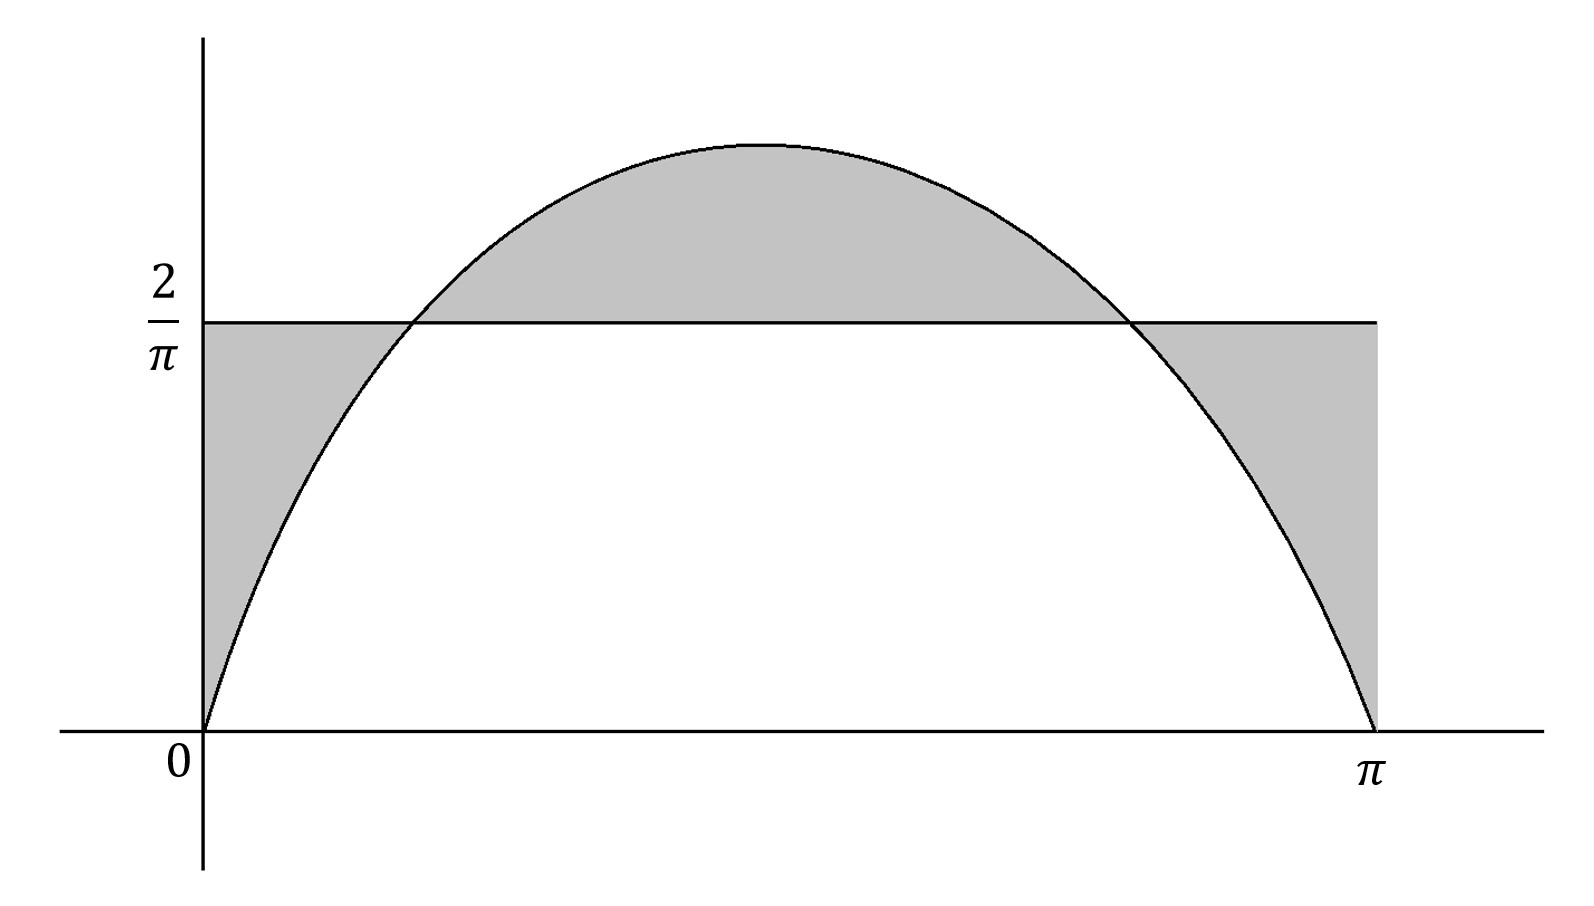
\includegraphics[scale=0.15]{mnk_geo_final.jpg}
        \caption{Z MNK želimo minimizirati ploščino sivega območja.}
    \end{figure}
\end{ex}

\begin{ex}
    Točke $(1, 2), (2, 3), (3, 5), (4, 8)$ aproksimiraj po MNK s premico.

    Rešitev:
    $S = \Pp_1 = Lin\{1, x\}$
    \begin{equation*}
        \innerproduct{f}{g} = \sum_{i = 1}^{4} f(x_i), g(x_i) \text{, } x =
        \begin{bmatrix}
            1 \\
            2 \\
            3 \\
            4
        \end{bmatrix}
    \end{equation*}
    $f$, ki jo aproksimiramo, je znana le v točkah $\textbf{x}$.

    Izračunamo:
    \begin{align*}
        \innerproduct{1}{1} =& \sum_{i = 1}^{4}1\cdot 1 = 4 \\
        \innerproduct{1}{x} =& \sum_{i = 1}^{4}1\cdot x_i = 10 \\
        \innerproduct{x}{x} =& \sum_{i = 1}^{4}x_i^2 = 30 \\
        \innerproduct{f}{1} =& \sum_{i = 1}^{4} y_i \cdot 1 = 18 \\
        \innerproduct{f}{x} =& \sum_{i = 1}^{4} y_i x_i = 55
    \end{align*}

    Dobimo sistem
    \begin{equation*}
        \begin{bmatrix}
            4 & 10 \\
            10 & 30
        \end{bmatrix}
        \begin{bmatrix}
            \alpha_1 \\
            \alpha_2
        \end{bmatrix}
        =
        \begin{bmatrix}
            18 \\
            55
        \end{bmatrix}
    \end{equation*}
    iz katerega dobimo rezultat
    \[ \alpha = 
        \begin{bmatrix}
            -\frac{1}{2} \\
            2
        \end{bmatrix}\]

    Geometrijska interpretacija rešitve:
    \begin{equation*}
        \min_{p \in \Pp_1} \norm{f - p}_2 =\sqrt[]{\sum_{i = 1}^{4} (y_i -p(x_i))^2}
    \end{equation*}
    \begin{figure}[h]
        \center
        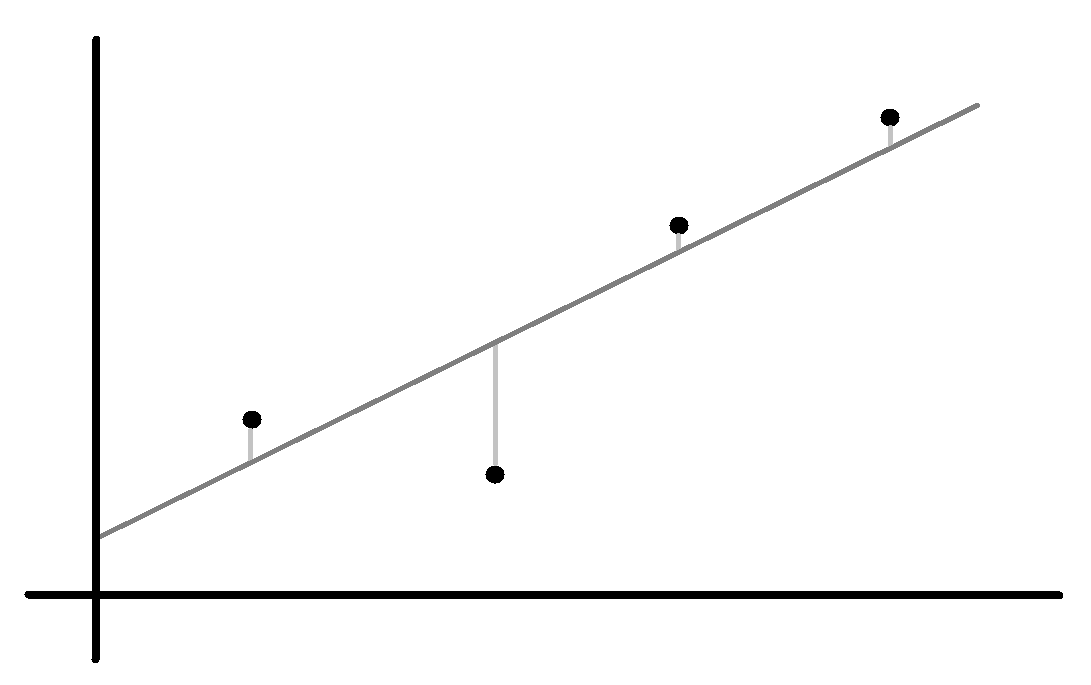
\includegraphics[scale=0.25]{mnk_geo_druga.png}
        \caption{Z MNK želimo najti temnosivo premico, ki minimizira svetlosive razdalje.}
    \end{figure}
\end{ex}
%\newpage
\subsubsection{Povezava s predoločenimi sistemi enačb}
\begin{equation*}
    Ax = b \text{, } A\in \R^{m \times n} \text{, } A = 
    \begin{bmatrix}
        a_1 & a_2 & \dots & a_n
    \end{bmatrix} \text{, }  b \in R^m
\end{equation*}
\begin{equation*}
    \min_{x \in \R^n} \norm{Ax - b}_2 = \min_{z \in ImA} \norm{b - z}
\end{equation*}

Aproksimiramo vektor $b \in \R^m (X = \R^m)$
\begin{equation*}
    S = Lin\{a_1, a_2, \dots, a_n\} = ImA
\end{equation*}
\begin{equation*}
    b^* = \sum_{j = 1}^{n}x_j a_j = Ax
\end{equation*}
\begin{equation*}
    \innerproduct{x}{y} = \sum_{i = 1}^{m}x_i y_i = x^T y
\end{equation*}

$\innerproduct{x}{y} = \sum_{i = 1}^{m} x_i y_i$:
\begin{equation}
    G = (\innerproduct{a_j}{a_i})_{i, j = 1}^n = A^T A
\end{equation}
\begin{equation}
    \text{desna stran } = (\innerproduct{a_i}{b})_{i = 1}^n = A^Tb
\end{equation}

\begin{ex}
    $X = \mathscr{C} ([0, 1])$
    \begin{equation*}
        S = P_{n-1} = Lin\{1, x, x^2, \dots, x^{n-1}\}
    \end{equation*}
    \begin{equation*}
        \innerproduct{f}{g} = \int_{0}^{1} f(x) g(x) dx
    \end{equation*}
    \begin{equation*}
        \innerproduct{\varphi_i}{\varphi_j} = \int_{0}^{1} x^{i-1} x^{j-1} dx = \int_{0}^{1}x^{i+j-2} dx = \frac{1}{i+j-1}
    \end{equation*}
    \begin{equation*}
        G = (\frac{1}{i+j-1})_{i, j = 1}^n
    \end{equation*}
    kjer je G Hilbertova matrika. Te so zelo občutljive.
\end{ex}

% 24. 2. 2023

Gramova matrika je lahko zelo občutljiva. Reševanju sistema linearnih enačb se izognemo, če v podprostoru $S$ izberemo $\textbf{ortonormirano bazo}$:
\begin{equation*}
    \{\varphi_1, \varphi_2, \dots, \varphi_n\}
\end{equation*}
je ortonormirana baza, če
\begin{equation*}
    \varphi_1 \perp \varphi_j \text{ } \forall i \neq j \text{ in } \norm{\varphi_i}_2 = 1
\end{equation*}
V tem primeru je $G = I$ in $\alpha_i = \innerproduct{f}{\varphi_i}$,  $f^* = \sum_{i = 1}^{n}\innerproduct{f}{\varphi_i} \varphi_i$. Ortonormirano
bazo izračunamo z $\textbf{modificiranim Gram-Scmidtovim algoritmom}$.

\begin{algorithm}
    \caption{Modificiran Gram-Schmidtov algoritem}\label{alg:mgs}
    \hspace*{\algorithmicindent} \textbf{Input} baza $\{\psi_1, \psi_2, \dots, \psi_n\}$
    \begin{algorithmic}[1]
        \For{$i = 1:n$}
            \State $\varphi_i = \psi_i$
        \EndFor
        \For{$i = 1:n$}
            \State $\varphi_i = \frac{\varphi_i}{\norm{\varphi_i}_2}$
            \For{$j = i+1:n$}
                \State $\varphi_j = \varphi_j - \innerproduct{\varphi_j}{\varphi_i}\varphi_i$
            \EndFor
        \EndFor
    \end{algorithmic}
    \hspace*{\algorithmicindent} \textbf{Output} ortonormirana baza $\{\varphi_1, \varphi_2, \dots, \varphi_n\}$
\end{algorithm}


$X \in \mathscr{C}([a, b])$
\begin{figure}[h]
    \center
    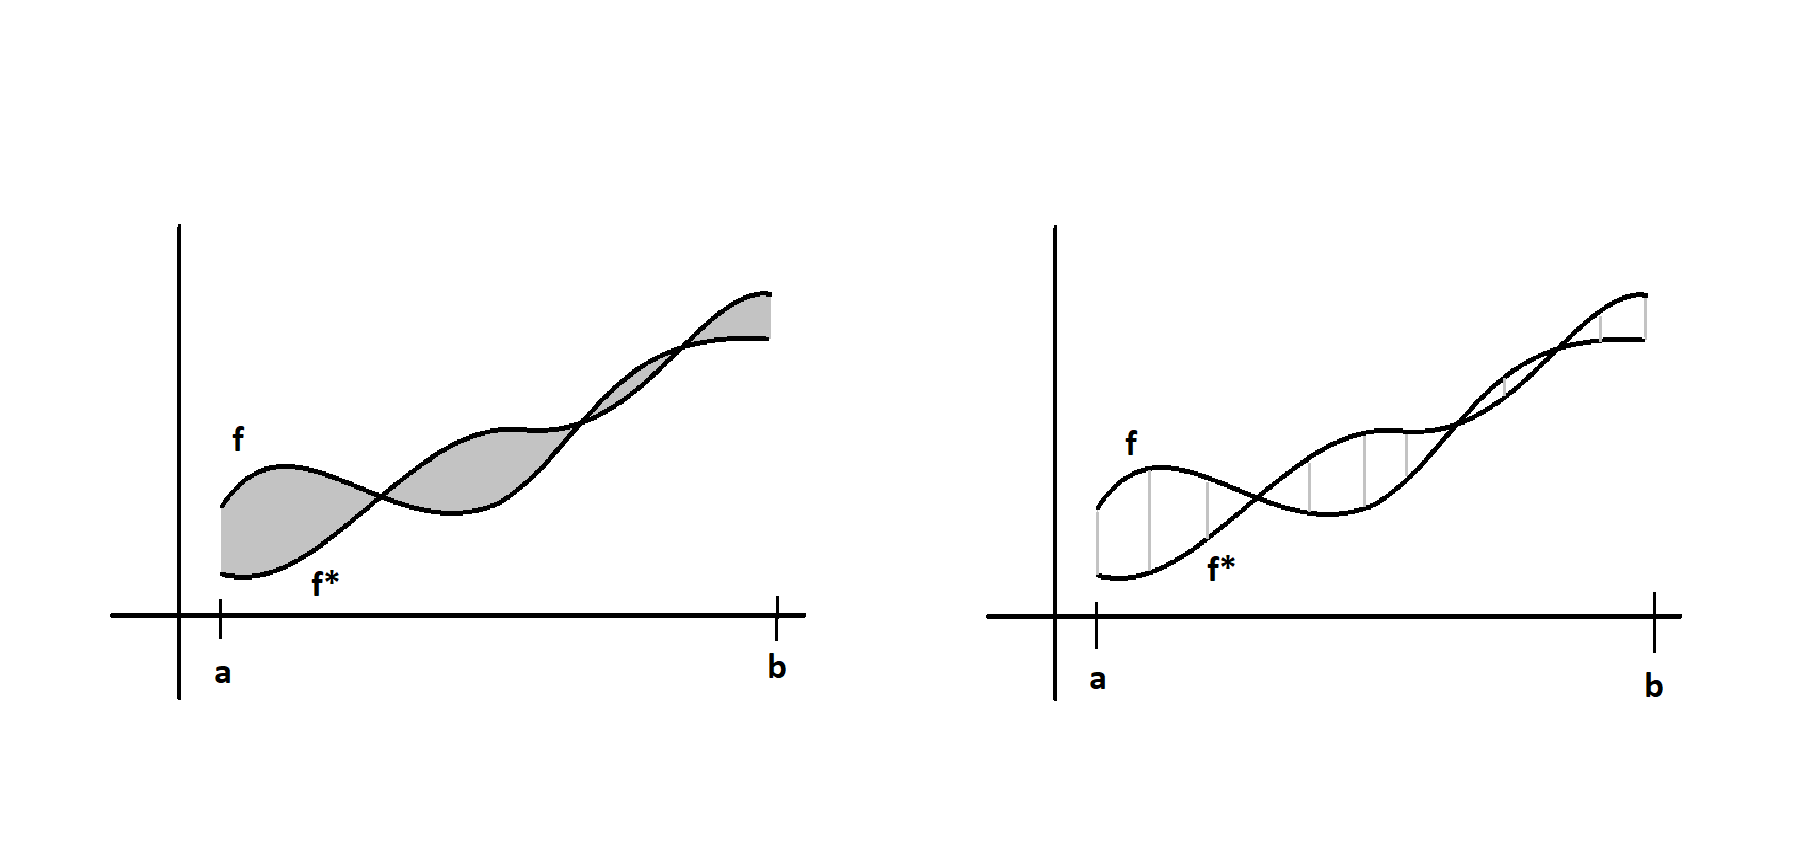
\includegraphics[scale=0.25]{mnk_tretja.png}
    \caption{Druga norma, porojena iz zveznega (levo) in diskretnega (desno) skalarnega produkta}
\end{figure}

\subsection{Enakomerna aproksimacija zveznih funkcij s polinomi}
\begin{equation*}
    X = \mathscr{C} ([a, b]), S = \Pp_n, \norm{\cdot}_{\infty}
\end{equation*}

Problem: Za dano funkcijo $f \in \mathscr{C} ([a, b])$ iščemo polinom $p^* \in \Pp_n$, za katerega velja
\begin{equation*}
    \norm{f - p^*}_{\infty, [a, b]} = \min_{p \in \Pp_n} \norm{f - p}_{\infty, [a, b]} = \min_{p \in Pp_n} \max_{x \in [a, b]} \left| f(x) - p(x) \right|
\end{equation*}
$p^*$ imenujemo $\textbf{polinom najboljše enakomerne aproksimacije (PNEA)}$.
Problem je nelinearen.

(vstavi skico)

Nasledni izrek nam poda $\textbf{zadostni pogoj}$, da je nek polinom PNEA za neko funkcijo.
\begin{theorem}
    Naj bo $f \in \mathscr{C}([a, b])$. Če je polinom $p \in \Pp_n$ tak, da $\textbf{residual}$
    \begin{equation}
        r = f - p
    \end{equation}
    alternirajoče doseže svojo normo $\norm{p}_{\infty, [a, b]}$ v vsaj $n + 2$ različnih točkah $(x_i)_{i=0}^{n+1}$
    \[a \leq x_0 < x_1 < \dots < x_{n+1} \leq b\]
    Potem je $p$ polinom najboljše enakomerne aproksimacije za $f$ na $[a, b]$.
\end{theorem}

\rem{Kaj pomeni "alternirajoče doseže svojo normo"?}
\begin{equation*}
    \norm{r}_{\infty, [a, b]} = \left| r(x_i) \right| \forall i \in [n]
\end{equation*}
in
\begin{equation*}
    r(x_i)r(x_{i+1}) < 0 \forall i
\end{equation*}

(vstavi graf)

\begin{proof}
    Dokaz s protislovjem.

    Recimo, da $p$ ne bi bil PNEA za $f$. Tedaj bi obstajal nek drug polinom $q \in \Pp_n$, da bi veljalo
    \begin{align*}
        \left| f(x_i) - q(x_i) \right| \leq& \max_{x \in [a, b]} \left| f(x) - q(x) \right| \\
                             =& \norm{f - q}_{\infty, [a, b]} \\
                             <& \norm{f - p}_{\infty, [a, b]} \\
                             =& \left| f(x_i) - p(x_i) \right| \text{  } \forall i = 0, 1, 2, \dots, n+1
    \end{align*}
    Torej za $\forall i $ velja:
    \begin{equation*}
        \left| f(x_i) - q(x_i) \right| < \left| f(x_i) - p(x_i) \right|
    \end{equation*}
    To razvijemo v neenakosti
    \begin{equation*}
        - sign(f(x_i) - p(x_i)) (f(x_i) - p(x_i)) < f(x_i) - q(x_i)
    \end{equation*}
    in
    \begin{equation*}
        f(x_i) - q(x_i) < sign(f(x_i) - p(x_i)) (f(x_i) - p(x_i))
    \end{equation*}
    Če v neenakostih $x_i$ spremenimo v $x_{i+1}$ ter upoštevamo enakost
    \begin{equation*}
        sign(f(x_{i+1}) - p(x_{i+1})) = - sign(f(x_i) - p(x_i))
    \end{equation*}
    dobimo neenakosti
    \begin{equation*}
        sign(f(x_i) - p(x_i)) (f(x_{i+1}) - p(x_{i+1})) < f(x_{i+1}) - q(x_{i+1})
    \end{equation*}
    in
    \begin{equation*}
        f(x_{i+1}) - q(x_{i+1}) < - sign(f(x_i) - p(x_i)) (f(x_{i+1}) - p(x_{i+1}))
    \end{equation*}

    Brez škode za splošnost (BŠS) lahko rečemo, da je $sign(f(x_i) - p(x_i)) = 1$. Potem je $f(x_i) - q(x_i) < f(x_i) - p(x_i)$, $p(x_i) - q(x_i) < 0$ in
    $f(x_{i+1}) - p(x_{i+1}) < f(x_{i+1}) - q(x_{i+1})$, torej $p(x_{i+1}) - q(x_{i+1}) > 0$.

    Vidimo, da ima razlika $p-q$ ničlo na intervalu $(x_i, x_{i+1})$ za $i \in [n]$. Razlika $p-q$ je polinom stopnje $n$, ki ima $n+1$ ničel.
    Torej mora biti $p \equiv q$.
\end{proof}

Izkaže se, da je pogoj tudi potreben (torej da velja ekvivalenca), a je dokaz težek, zato ga bomo izpustili.

Iskanje/računanje PNEA se prevede na iskanje ustrezne množice točk $\{x_i, a \leq x_0 < x_1 < \dots < x_{n+1} \leq b\}$.

\begin{defn}
    Naj bo $E = \{x_i, a \leq x_0 < x_1 < \dots < x_{n+1} \leq b\}$. Definirajmo $\textbf{minimaks}$ za $f$ na $E$ konstruirati
    \begin{equation*}
        M_n (f, E) = \min_{p \in \Pp_n} \max_{x_i \in E} \left| f(x_i) - p(x_i) \right|
    \end{equation*}
\end{defn}

Polinom, pri katerem je ta minimum dosežen, imenujemo $\textbf{polinom}$ $\textbf{najboljše}$ $\textbf{enakomerne}$ $\textbf{aproksimacije}$ $\textbf{za}$ $f$
$\textbf{na}$ $\textbf{množici}$ $E$. Izračunamo ga tako,
da rešimo naslednji sistem linearnih enačb: (brez izpeljave)
\begin{equation*}
    f(x_i) - p(x_i) = (-1)^i m, i \in [n+1] 
\end{equation*}

Imamo torej $n+2$ enačb in $n+2$ neznank ($n + 1$ v polinomu $p$ in eno v $m$):
\begin{equation*}
    p(x) = \sum_{j = 0}^{n} a_j x^j
\end{equation*}
ter koeficient $m$, za katerega velja
\begin{equation*}
    \left| m \right| = M_n (f, E)
\end{equation*}

(vstavi slikco)

\section{Interpolacija}
Problem: Podane imamo vrednosti izbrane funkcije $f$ v $n+1$ paroma različnih točkah $x_0, x_1, \dots, x_n$ na realni osi. Te točke bomo imenovali
$\textbf{interpolacijske}$ $\textbf{točke}$. Iščemo neko preprostejšo funkcijo $g$, ki zadošča pohojem
\begin{equation*}
    g(x_i) = f(x_i) \forall i \in [n]
\end{equation*}
$g$ imenujemo $\textbf{interpolacijska}$ $\textbf{funkcija}$. Za interpolacijske funkcije običajno izberemo polinome, odsekoma polinomske funkcije \dots


% 27.2.2023
Interpolacija se uporablja za
\begin{itemize}
    \item aproksimacijo dane funkcije
    \item kadar funkcijo $f$ poznamo le v točkah $x_0, x_1, \dots, x_n$, radi pa bi izračunali vrednost te funkcije tudi za $x$, ki ni ena izmed interpolacijskih točk.
    \item za izpeljavo formul za numerično integriranje, odvajanje, reševanje navadnih diferencialnih enačb (NDE) \dots
\end{itemize}

\subsection{Polinomska interpolacija}
Za $f \in \mathscr{C}([a, b])$ in interpolacijske točke $a \leq x_0 < x_1 < \dots < x_m \leq b$ iščemo $\textbf{polinom}$ $p_i$, ki zadošča enačbam
\begin{equation*}
    p(x_i) = f(x_i), i = a, \dots, n
\end{equation*}
Enačb je $n+1$. Da dobimo enako število enačb, moramo izbrati $p \in \Pp_n$.

\begin{equation*}
    p(x) = a_0 + a_1 x + a_2 x^2 + \dots + a_n x^n
\end{equation*}

Enačbe (za $i = 0, 1, \dots, n$)
\begin{equation*}
    a_0 + a_1 x_i + a_2 x_i^2 + \dots + a_n x_i^n
\end{equation*}
lahko zapišemo matrično
\begin{equation*}
    \begin{bmatrix}
        1 & x_0 & x_0^2 & \dots & x_0^n \\
        1 & x_1 & x_1^2 & \dots & x_1^n \\
    \vdots & \vdots & \vdots &  & \vdots \\
        1 & x_n & x_n^2 & \dots & x_n^n 
    \end{bmatrix}
    \begin{bmatrix}
        a_0 \\
        a_1 \\
        \vdots \\
        a_n
    \end{bmatrix}
    =
    \begin{bmatrix}
        f(x_0) \\
        f(x_1) \\
        \vdots \\
        f(x_n) \\
    \end{bmatrix}
\end{equation*}
Matriko, ki jo uporabimo, imenujemo $\textbf{vandermondova matrika}$.
\begin{equation*}
    \det V(x_0, x_1, \dots, x_n) = \prod_{0 \leq i < j \leq n} (x_j - x_i)
\end{equation*}

Ker je Vandermondova matrika obrnljiva, sledi, da imamo enolično rešitev. Torej obstaja $\textbf{enoličen}$ polinom stopnje $n$, ki interpolira $n+1$ paroma
različnih točk.
Tak interpolacijski problem imenujemo $\textbf{korenten}$ interpolacijski problem.
Vandermondova matrika je primer $\textbf{zelo občutljive}$ matrike.
Poleg tega nimamo rešitve v $\textbf{zaključeni obliki}$.
Spoznali bomo dva druga zapisa interpolacijskega polinoma:
\begin{itemize}
    \item Lagrangeva oblika zapisa
    \item Newtonova oblika zapisa
\end{itemize}

\subsubsection{Lagrangeva oblika zapisa interpolacijskega polinoma}
Definiramo naslednje polinome:
\begin{align*}
    \ell_{0, n} (x) =& \frac{(x-x_1)(x-x_2) \dots (x - x_n)}{(x_0 - x_1)(x_0 - x_2) \dots (x_0 - x_n)} \\
    \ell_{1, n} (x) =& \frac{(x-x_1)(x-x_2) \dots (x - x_n)}{(x_1 - x_0)(x_1 - x_2) \dots (x_1 - x_n)} \\
    \vdots &\\
    \ell_{n, n} (x) =& \frac{(x-x_1)(x-x_2) \dots (x - x_n)}{(x_n - x_0)(x_n - x_1) \dots (x_n - x_{n-1})}
\end{align*}

oziroma
\begin{equation*}
    \ell_{i, n} (x) = \prod_{j = 0, j \neq i}^{n} \frac{(x - x_j)}{(x_i - x_j)}
\end{equation*}
za $i = 0, 1, \dots, n$. To imenujemo $\textbf{Lagrangevi bazni polinomi}$.

Velja:
\begin{equation*}
    \ell_{i, n} (x) = \delta_{i, j} = \begin{cases}
        1 &; i = j \\
        0 &; i \neq j
    \end{cases}
\end{equation*}
Vsi ti polinomi so stopnje točno $n$.

\begin{theorem}
    Polinomi $\ell_{i, n}$ za $i = 0, 1, \dots, n$ so baza za $\Pp_n$.
\end{theorem}

\begin{proof}
    Dokazati moramo le, da so linearno neodvisni. Preveriti moramo, da je $\alpha_0 \ell_{i, n} +  \alpha_1 \ell_{i, n} + \dots +
    \alpha_n \ell_{i, n} = 0 <=> \alpha_0 = \alpha_1 = \dots = \alpha_n = 0$.

    ($\Longrightarrow$)
    \begin{equation*}
        \sum_{j = 0}^{n} \alpha_j \ell_{j, n} (x) = 0 \text{ }\forall x
    \end{equation*}
    Vstavimo $x = x_i$ in dobimo
    \begin{equation*}
        0 = \sum_{j = 0}^{n} \alpha_j \ell_{j, n} (x_i) = \sum_{j = 0}^{n} \alpha_j \delta_{i, j} = \alpha_i
    \end{equation*}
    ($\Longleftarrow$) Očitno.
\end{proof}

Iz dokaza izreka sledi, da lahko vsak polinom $p \in \Pp_n$ zapišemo kot linearno kombinacijo
\begin{equation*}
    p(x) = \sum_{j = 0}^{n} c_j \ell_{j, n} (x)
\end{equation*}
za $c_j \in \R$.

Kako izbrati koeficiente, da bo polinom interpolacijski oziroma da bo zadoščal pogojem
\begin{equation*}
    p(x_i) = \sum_{j = 0}^{n} c_j \ell_{j, n} (x_i) = f(x_i)
\end{equation*}
za $i = 1, \dots, n$. Za vsak $i$ je tudi vsota enaka $c_i$.

Dobili smo
\begin{equation*}
    p(x) = \sum_{j = 0}^{n} f(x_j) \ell_{j, n}(x)
\end{equation*}
kar je Lagrangeva oblika zapisa interpolacijskega polinoma.

\begin{ex}
    Naj bo $f(x) = e^x$. Pošiči interpolacijski polinom za $f$ na točkah $x_0 = 0, x_1 = 1, x_2 = 3, x_3 = 4$.
    Za $n = 3$ izračunamo

    \begin{align*}
        \ell_{0, 3}(x) =& \frac{(x-1)(x-3)(x-4)}{((0-1)(0-3)(0-4))} \\
                       =& -\frac{1}{12}(x-1)(x-3)(x-4) \\
        \ell_{1, 3}(x) =& \frac{x(x-3)(x-4)}{(1(1-3)(1-4))} \\
                       =& \frac{1}{6} x(x-3)(x-4) \\
        \ell_{2, 3}(x) =& \frac{x(x-1)(x-4)}{(3(3-1)(3-4))} \\
                       =& -\frac{1}{6} x(x-1)(x-4) \\
        \ell_{3, 3}(x) =& \frac{x(x-1)(x-3)}{(4(4-1)(4-3))} \\
                       =& \frac{1}{12} x(x-1)(x-3) \\
    \end{align*}

    in dobimo rešitev
    \begin{equation*}
        p(x) = e^0 \ell_{0, 3}(x) + e^1 \ell_{1, 3}(x) + e^3 \ell_{2, 3} (x) + e^4 \ell_{3, 3}(x)
    \end{equation*}
    Časovna zahtevnost za evaluacijo $\ell_{i, n}(x)$ v $x_i$ je $\mathcal{O}(n^2)$. Ker v praksi izpustimo skupen polinom,
    je končna časovna zahtevnost $\mathcal{O}(n)$, tako kot Hornerjev algoritem.
\end{ex}


\begin{lemma}
    Če je $f \in \Pp_n$, potem je $\sum_{i = 0}^{n} f(x_i) \ell_{i, n} (x) = f(x)$.
\end{lemma}
\begin{proof}
    Sledi iz enoličnosti interpolacijskega polinoma.
\end{proof}

\begin{conseq}
    \begin{equation}
        \sum_{i = 0}^{n} \ell_{i, n}(x) = 1
    \end{equation}
    Lagrangevi bazni polinomi tvorijo $\textbf{razčlenitev}$ oziroma $\textbf{razčlenitev enote}$, ki pozitivno vpliva na stabilnost baze.
\end{conseq}

\begin{theorem}[O napaki interpolacije.]
    Naj bodo $a \leq x_0 < x_1 \dots < x_n \leq b$, $f \in \mathscr{C}^{n+1}([a, b])$ in naj bo $p$ interpolacijski polinom za $f$ na teh točkah. Potem za vsak $x \in [a, b]$
    obstaja $\xi_x \in (a, b)$, da velja
    \begin{equation*}
        f(x) - p(x) = \omega (x) \frac{f^{(n+1)}(\xi_x)}{(n+1)!}
    \end{equation*}
    kjer velja
    \begin{equation*}
        \omega (x) = (x - x_0)(x-x_1) \dots (x - x_n)
    \end{equation*}
\end{theorem}

\begin{proof}
    Če je $x = x_i$, potem $f(x_i) - p(x_i) = 0$ in $\omega (x_i) = 0$ ter enakost velja za vsak $\xi_x \in (a, b)$. Naj bo sedaj $x \neq x_i$, $i = 0, 1, \dots, n$
    in naj bo ta $x$ fiksen.
    Definirajmo $F(u) = f(u) - p(u) - c \omega (u)$ za neko konstanto $c$, pri čemer za $F$ velja $F \in \mathscr{C}^{n+1}([a, b])$, $F(x_i) = f(x_i) - p(x_i) - c \omega (x_i) = 0$ za $i = 0, 1, \dots, n$.
    Konstanto $c$ izberemo tako, da bo tudi $F(x) = 0$. Torej ima $F$ na $[a, b]$ $n+2$ različnih ničel. Potem ima $F'$ na $(a, b)$ $n+1$ različnih ničel.
    Potem ima $F''$ na (a, b) n različnih ničel \dots Potem ima $F^{(n+1)}$ na $(a, b)$ vsaj eno ničlo. Označimo to ničlo z $\xi_x$. Torej je
    \begin{align*}
        0 =& F^{(n+1)}(\xi_x) \\
          =& f^{(n+1)}(\xi_x) - p^{(n+1)}(\xi_x) - c \omega ^{(n+1)}(\xi_x)
    \end{align*}
    Uporabimo razmislek od zgoraj in dobimo
    \begin{equation*}
        0 = f^{(n+1)}(\xi_x) - c (n+1)!
    \end{equation*}
    Ko to preuredimo, dobimo
    \begin{equation*}
        c = \frac{1}{(n+1)!}f^{(n+1)}(\xi_x)
    \end{equation*}
\end{proof}

Za poljuben $c \in [a, b]$ po izreku velja
\begin{equation*}
    \left| f(x) - p(x) \right| = \left| \omega \right| \frac{1}{(n+1)!} \left| f^{(n+1)}(\xi_x) \right| \leq \norm{\omega}_{\infty, [a, b]} \frac{1}{(n+1)!} \norm{f^{(n+1)}}_{\infty, [a, b]}
\end{equation*}
Iz tega sledi
\begin{equation*}
    \norm{f - p}_{\infty, [a, b]} \leq \frac{1}{(n+1)!} \norm{\omega}_{\infty, [a, b]} \norm{f^{(n+1)}}_{\infty, [a, b]}
\end{equation*}
Ta ocena je uporabna v teoriji, ne pa tudi v praksi.

Lagrangeva oblika je zaradi enostavnosti zelo uporabna pri izpeljavi formul za numerično integracijo, odvajanje \dots, ima pa tudi nekaj pomankljivosti pri praktični uporabi:
\begin{itemize}
    \item numerično računanje vrednosti polinoma v Lagrangevi obliki \dots
    \item Numerične težave, če so interpolacijske točke preblizu skupaj
    \item Konstrukcija ni rekurzivna. Dodajanje novih točk je zahtevno.
\end{itemize}

\subsubsection{Newtonova oblika zapisa interpolacijskega polinoma}
Za bazo, v kateri bomo predstavili interpolacijski polinom, izberemo $\\ \textbf{prestavljene}$ $\textbf{potence}$. % previdno z \\
\begin{equation*}
    \{1, x-x_0, (x-x_0)(x-x_1), \dots, (x-x_0) (x-x_1) \dots (x-x_n)\}
\end{equation*}
Očitno je to baza: vidimo, da se stopnje povečujejo in je posledično kolokacijska matrika spodnje trikotna. V nadaljevanju bomo naredili rekurzivno konstrukcijo.

% 6. 3. 2023
Vsak $p \in \Pp_n$ lahko zapišemo kot 
\begin{equation*}
    \sum_{i = 0}^{n} \bigl( c_i \prod_{j = 0}^{i-1} (x-x_j) \bigr)
\end{equation*}
Iščemo koeficiente $(c_i)_{i=0}^n$, da bo $p$ interpolacijski.
Ta $p$ bomo konstruirali $\textbf{rekurzivno}$.
Naj bo $p_{k-1}$ interpolacijski polinom za $f$ na točkah $x_0$, $x_1$, $\dots$, $x_{k-1}$. Kako poiskati $p_k$, ki bo interpolacijski za $f$ na točkah
$x_0, x_1, \dots, x_k$, kjer bo $p_{k-1} \in \Pp_{k-1} \text{ in } p_k \in \Pp_k$?

\begin{equation*}
    p_k (x) = p_{k-1}(x) + c (x-x_0)(x-x_1)\cdots(x-x_{k-1})
\end{equation*}
Vstavimo $x = x_j$, $j \in \{0, 1, \dots, k-1\}$
\begin{equation*}
    p_k(x_j) = p_{k-1}(x_j) + c \cdot 0 = f(x_j)
\end{equation*}
Ostane le pogoj za $x = x_k$
\begin{equation*}
    p_k(x_k) = f(x_k)
\end{equation*}
kjer lahko zapišemo
\begin{equation*}
    p_k(x_k) = p_{k-1}(x_x) +  c \prod_{j = 0}^{k-1}(x_k - x_j)
\end{equation*}
S tem je določen $c$, ki je kar $\textbf{vodilni koeficient}$ od $p_k$. Označimo ga z $[x_0, x_1, \dots, x_k] f$ in ga imenujemo $\textbf{deljena diferenca}$.

\begin{defn}
    $\textbf{Deljena diferenca}$  $[x_0, x_1, \dots, x_k] f$ je vodilni koeficient interpolacijskega polinoma stopnje $k$ (koeficient pri $x^k$) za funkcijo $f$ na
    točkah $x_0, x_1, \dots, x_k$.
\end{defn}

Sledi, da lahko $p_k(x)$ zapišemo kot
\begin{equation*}
    p_k(x) = p_{k-1}(x) + [x_0, x_1, \dots, x_k]f \cdot (x-x_0)(x-x_1) \dots (x-x_{k-1})
\end{equation*}

(vstavi graf)
V grafu: $p_0 \in \Pp_p$, $p_0(x) = x_0 \cdot 1$.
Po definiciji je $[x_0]f = f(x_0)$.

Iz te rekurzivne konstrukcije dobimo
\begin{align*}
    p_n(x) = & p_{n-1}(x) + [x_0, x_1, \dots, x_n] f (x-x_0)(x-x_1) \dots (x-x_{n-1}) \\
           = & \dots \\
           = & p_o(x) + [x_0, x_1] f (x-x_0) + [x_0, x_1, x_2] f (x-x_0)(x-x_1) + \\
            & + \dots + [x_0, x_1, \dots, x_n] f (x-x_0)(x-x_1) \dots (x-x_{n-1})
\end{align*}
\begin{equation*}
    p_n(x) = \sum_{i = 0}^{n}[x_0, x_1, \dots, x_i] f (x-x_0)(x-x_1)\dots(x-x_{i-1})
\end{equation*}

Temu rečemo $\textbf{Newtonova oblika}$ zapisa interpolacijskega polinoma.

Kako izračunati deljene diference?

\begin{itemize}
    \item $[x_0] f = f(x_0)$
    \item $[x_0, x_1] f = \text{?}$
\end{itemize}

(vstavi graf)

\begin{align*}
    p_1 (x) =& f(x_0) + \frac{f(x_1)- f(x_0)}{x_1 - x_0} (x-x_0) \\
            =& [x_0] f \cdot 1 + [x_0, x_1] f (x-x_0)
\end{align*}
V zgornji enačbi je $\frac{f(x_1)- f(x_0)}{x_1 - x_0}$ vodilni koeficient, $1$ in $(x-x_0)$ pa sta baza. Iz tega sledi
\begin{equation*}
    [x_0, x_1] f = \frac{f(x_1)- f(x_0)}{x_1 - x_0} = \frac{[x_1]f - [x_0]f}{x_1 - x_0}    
\end{equation*}



\begin{theorem}[Rekurzivna formula za deljene diference]
    Naj bodo $x_0, x_1, \dots, x_k$ paroma različne točke. Tedaj velja
    \begin{equation*}
        [x_0, x_1, \dots, x_k]f = \frac{[x_1, x_2, \dots x_k] f - [x_0, x_1, \dots x_{k-1}]f}{x_k - x_0}
    \end{equation*}
\end{theorem}

\begin{rem}
    Pazi na koeficiente! V števcu gredo pri prvem od $x_1$ do $x_k$, pri drugem pa od $x_0$ do $x_{k-1}$. Tista, ki smo ju izpustili,
    potem odštejemo v imenovalcu, torej $x_k-x_0$.
\end{rem}

\begin{proof}
    Naj bo $q_0$ interpolacijski za $f$ na točkah $x_0, x_1, \dots, x_{k-1}$ in $q_1$ interpolacijski za $f$ na točkah $x_1, x_2, \dots, x_k$.
    Velja, da sta $q_0, q_1 \in \Pp_{k-1}$.
    Kako priti do polinoma $p$, ki bo interpolacijski na $x_0, x_1, \dots, x_k$? Ta $p$ bo tak, da bo veljalo $p \in \Pp_k$.

    Sestavimo model za $p$
    \begin{equation*}
        p(x) = \ell_0(x) q_0(x) + \ell_1(x) q_1(x), \ell_0, \ell_1 \in \Pp_1, \ell_0, \ell_1 = ?
    \end{equation*}
    \begin{equation*}
        x = x_j, j \in \{x_1, x_2, \dots, x_{k-1}\}
    \end{equation*}
    Dobimo tri pogoje:
    \begin{itemize}

        \item[($\star \star$)] $x = x_j$
        \begin{equation*}
            p(x_j) = \ell_0(x_j) q_0 (x_j) + \ell_1 (x_j) q_1 (x_j) = (\ell_0 (x_j) + \ell_1 (x_j)) f(x_j) \stackrel{\text{?}}{=} f(x_j)
        \end{equation*}

        \item[($\star$)] $x = x_0$
        \begin{equation*}
            p(x_0) = \ell_0(x_0) f(x_0) + \ell_1 (x_0) q(x_0) \stackrel{\text{?}}{=} f(x_0)
        \end{equation*}

        \item[($\star$)] $x = x_k$
        \begin{equation*}
            p(x_k) = \ell_0 (x_k) q(x_k) + \ell_1(x_k) f(x_k) \stackrel{\text{?}}{=} f(x_k)
        \end{equation*}

    \end{itemize}
    
    Če izberemo
    \begin{equation*}
        \ell_0(x) = \frac{x - x_k}{x_0 - x_k}
    \end{equation*}
    in
    \begin{equation*}
        \ell_1(x) = \frac{x - x_0}{x_k - x_0}
    \end{equation*}
    zadostimo pogojema ($\star$). Ker pa je $\ell_0(x) + \ell_1(x) = 1$ za $\forall x$, pa velja tudi ($\star \star$).

    Torej
    \begin{equation*}
        p(x) = \frac{x-x_k}{x_0-x_k} q_0(x) + \frac{x-x_0}{x_k-x_0} q_1(x)
    \end{equation*}
    \begin{rem}
        V nadaljevanju se bo namesto vodilni koeficient pisalo $v.k.$
    \end{rem}
    Primerjamo vodilne koeficiente na levi in desni strani in dobimo:
    \begin{equation*}
        v.k.(p) = [x_0, x_1, \dots, x_k]f
    \end{equation*}
    Na desni strani:
    \begin{equation*}
        \frac{1}{x_0-x_k} \cdot v.k. (q_0) + \frac{1}{x_k - x_0} \cdot v.k. (q_1) = \frac{[x_1, x_2, ..., x_k] f - [x_0, x_1, ..., x_{k-1}] f}{x_k - x_0}
    \end{equation*}
\end{proof}

\subsubsubsection{Trikotna shema}
\begin{equation*}
    [x_0, x_1, x_2] f = \frac{[x_1, x_2]f - [x_0, x_1] f}{x_2 - x_0}
\end{equation*}
Deljive diference, ki jih potrebujemo v zapisu interpolacijskega polinoma, računamo v $\textbf{trikotni shemi}$ (primer za $n = 3$):
(vstavi shemo)
%\begin{tabular}{ c c c }
%    \cdot & [\cdot] f & [\cdot, \cdot]f \\ 
%    x_0 & [x_0] f & cell6 \\  
%    x_1 & [x_1] f & cell9     \\
%    x_2 & [x_2] f &       \\
%    x_3 & [x_3] f &
%\end{tabular}


\begin{ex}
    Poišči polinom $p$, za katerega velja $p(0) = 1$, $p(1) = 3$, $p(3) = 5$ in $p(4) = 2$.

    $p \in \Pp_3$, $x_0 = 1, x_1 =3,  x_2 = 5, x_3 = 4$
    baza:
    \begin{equation*}
        \{1, x, x(x-1), x(x-1)(x-3)\}
    \end{equation*}
    (tabela)
    \begin{equation*}
        p(x) = 1 \cdot 1 + 2 \cdot x - \frac{1}{3} \cdot x(x-1) - \frac{1}{4} \cdot x(x-1)(x-3)
    \end{equation*}
\end{ex}

Za splošen $n$:
(shema)

Kako izračunati vrednost polinoma v Newtonovi bazi pri izbranem $x$?

Označimo $d_i = [x_0, x_1, \dots, x_i] f, i = 0, 1, \dots, n$
$n = 4$
\begin{align*}
    p(x) =& d_0 \cdot 1 + d_1 (x-x_0) + d_2 (x-x_0)(x-x_1) + \\
         +& d_3 (x-x_0)(x-x_1)(x-x_2) + d_4 (x-x_0)(x-x_1)(x-x_2)(x-x_3) \\
         =& d_0 + (x-x_0)(d_1 - (x-x_1)(d_2 - (x-x_2)(d_3 - (x-x_3)d_4)))
\end{align*}
zapišemo
\begin{align*}
    v_4 =& d_4 \\
    v_3 =& d_3 + (x-x_3)v_4 \\
    v_2 =& d_2 + (x-x_2)v_3 \\
    v_1 =& d_1 + (x-x_1)v_2 \\
    v_0 =& d_0 + (x-x_0)v_1
\end{align*}



\begin{algorithm}
    \caption{Posplošen Hornerjev algoritem}\label{alg:horner}
    \hspace*{\algorithmicindent} \textbf{Input} $\underline{d} (= [d_0, d_1, \dots, d_n]), \underline{x}(= [x_0, x_1, \dots..., x_n]), x$
    \begin{algorithmic}
        \State $v_n = d_n$
        \For{$i = n-1:-1:0$}
            \State $v_i = d_i + (x-x_i) v_{i+1}$
        \EndFor
        \State $v_0 = p(x)$
    \end{algorithmic}
    \hspace*{\algorithmicindent} \textbf{Output} $v_0$
\end{algorithm}

% pazi, da bo tabelca na pravem mestu
(tabelca za hronerja)

% 13. 3. 2023
Poglejmo si za $n = 1$

(slikca)

\begin{align*}
    p(x) =& f(x_0)\cdot 1 + [x_0, x_1] f (x-x_0) \\
         =& f(x_0) + \frac{f(x_1) - f(x_0)}{x_1 - x_0}(x-x_0) - (x_1 \to x_0) \\
         \longrightarrow& f(x_0) + \biggl(\lim_{x_1 \to x_0} \frac{f(x_1)-f(x_0)}{x_1-x_0}\biggr)(x-x_0)
    p(x) =& f(x_0) - f'(x_0)(x-x_0) \\
\end{align*}
Iz tega dobimo sistem enačb:
\begin{align*}
    p(x_0) =& f(x_0) \\
    p'(x_0) =& f'(x_0)
\end{align*}

\begin{defn}
    Pravimo, da se polinom $p$ s funkcijo $f$ ujema v točki $x_i$ ($k+1$)-kratno, če se ujema v vrednosti in prvih $k$ odvodih.
    Enačbe, ki določajo te pogoje:
    \begin{align*}
        p(x_i) =& f(x_i) \\
        p'(x_i) =& f'(x_i) \\
        p''(x_i) =& f''(x_i) \\
        \vdots& \\
        p^{(k)}(x_i) =& f^{(k)}(x_i)
    \end{align*}
    Tak polinom je Taylorjev polinom:
    \begin{equation*}
        p(x) = f(x_i) + f'(x_i)(x-x_i) + \frac{f''(x_i)}{2!}(x-x_i)^2 + \dots + \frac{f^{(k)}(x_i)}{k!}(x-x_i)^k
    \end{equation*}
    Če bomo v točki $x_i$ zahtevali $(k+1)$-kratno ujemanje, potem bomo to točko podali $(k+1)$-kratno:
    \begin{equation*}
        x_{i-1} < x_i = x_{i+1} = x_{i+2} = \dots x_{i+k} < x_{i+k+1}
    \end{equation*}
\end{defn}

\subsubsubsection{Posplošitev deljene diference}
Poglejmo si, kako posplošimo deljenje diference.
\begin{equation*}
    [x_i, x_i, \dots, x_i] f = \frac{f^{(k)}(x_i)}{k!}
\end{equation*}
\begin{rem}
    V zgornji enačbi imamo $(k+1)$ $x_i$-jev
\end{rem}

\subsubsubsection{Posplošitev rekurzivne formule}
\begin{rem}
    Vrstni red točk v deljeni diferenci $\textbf{ni}$ pomemben.
\end{rem}
Naj velja $x_i \leq x_{i+1} \leq x_{i+2} \leq \dots \leq x_{i+k}$. Potem je
\begin{equation*}
    [x_i, x_{i+1}, \dots, x_{i+k}] f =
    \begin{cases}
        \frac{f^{(k)}(x_i)}{k!} & x_i = x_{i+1} = \dots = x_{i+k} \\
        \frac{[x_{i+1}, \dots, x_{i+k}] f - [x_{i}, \dots, x_{i+k-1}]f}{x_{i+k} - x_{i}} & \text{sicer}
    \end{cases}
\end{equation*}

\begin{ex}
    Poišči polinom $p$, za katerega velja $p(0) = 1$, $p'(0) = 2$, $p''(0) = 3$, $p(1) = -1$, $p'(1) = 3$, $p(2) = 4$

    Določimo točke $x_0, x_1, \dots, x_5$:
    \begin{equation*}
        x_0 = 0, x_1 = 0, x_2 = 0, x_3 = 1, x_4 = 1, x_5 = 2
    \end{equation*}
    Potem sestavimo bazo:
    \begin{equation*}
        \{1, c, x^2, x^3, x^3(x-1), x^3(x-1)^2\}
    \end{equation*}
    Z uporabo trikotne sheme izračunamo koeficiente za polinom:
    (trikotna shema)
    Iz trikotne sheme preberemo koeficiente in sestavimo interpolacijski polinom:
    \begin{equation*}
        p(x) = 1 \cdot 1 + 2 \cdot x + \frac{3}{2} x^2 - \frac{11}{2}x^3 + \frac{29}{2}x^3(x-1) - \frac{79}{8} x^3(x-1)^2
    \end{equation*}
\end{ex}

Brez izpeljave povejmo še sledeče trditve:
\begin{claim}
    Za $f \in \mathscr{C}^k ([a, b]), a \leq x_0 \leq x_1 \leq x_n \leq b$, velja
    \begin{align*}
        [x_i, x_{i+1}, \dots, x_{i+k}] f = \frac{f^{(k)}(\xi)}{k!}, \xi \in [x_i, x_{i+k}]
    \end{align*}
\end{claim}


% pt2
\begin{claim}
    Za $f \in \mathscr{C}^{n+1}([a, b]), a \leq x_0 \leq x_1 \leq \dots \leq x_n \leq b$ in interpolacijski polinom $p$ za $f$ na teh točkah velja
    \begin{equation*}
        f(x) - p(x) = \omega(x) [x_0, x_1, \dots, x_n, x] f = \omega(x) \frac{f^{(n+1)(\xi_x)}}{(n+1)!}, \xi_x in (a, b), x \in [a, b]
    \end{equation*}
    \begin{equation*}
        \omega(x) = \prod_{i = 0}^{n} (x-x_i)
    \end{equation*}
\end{claim}

Kako izbrati interpolacijske točke na $[a, b]$? Obstaja več možnosti:
\begin{enumerate}
    \item Ekvidistantne točke:
    \begin{equation*}
        x_i = a + i \cdot h
    \end{equation*}
    kjer je $h = \frac{b-a}{n}$ in velja za $i = 0, 1, \dots, n$.

    (slikca)
    \item Čebiševe točke
    Izbira, pri kateri je neskončna norma polinoma $\omega$ najmanjša možna.
    \begin{equation*}
        \min_{a \leq x_0 < x_1 < \dots < x_n \leq b} \norm{\omega}_{\infty, [a, b]} = \min_{a \leq x_0 < x_1 < \dots < x_n \leq b} \max_{x \in [a, b]} | \omega(x) |
    \end{equation*}
    Rešitev so
    \begin{equation*}
        x_i = \frac{a+b}{2} + \frac{b-1}{2}\cos(\frac{2i+1}{2n+2}\pi)
    \end{equation*}
    za $i = 0, 1, \dots, n$
\end{enumerate}

Recimo, da izberemo $f \in \mathscr{C}([a, b])$, izberemo zaporedje interpolacijskih točk $(\{x_0, x_1, \dots, x_n\})_n$ in
povečujemo stopnjo $n$. Dobimo zaporedje interpolacijskih polinomov $(p_n)_n$. Zanima nas, kaj se dogaja z napako
\begin{equation}
    \norm{f-p}_{\infty, [a, b]} \xrightarrow{n \to \infty} ?? 
\end{equation}
Žal ne velja nujno, da bi šla ta napaka proti 0.

Protiprimer: (Rungejev primer)

Za funkcijo $f(x) = \frac{1}{1-x^2}$ na interalu $[-5, 5]$ interpoliramo z ekvidistantnimi točkami. Z večanjem $n$-ja gre napaka
proti $\infty$.

\subsubsubsection{Odsekoma polinomske funkcije (zlepki)}

IDEJA: Interval $[a, b]$ razdelimo na $m$ delov s stičnimi točkami 
\begin{equation*}
    a = x_0 < x_q < \dots < x_m = b
\end{equation*}

(slikca)

\begin{align*}
    s: [a, b] \to \R \\
    \restr{s}{[x_i, x_{i+1}]} \in \Pp_n
\end{align*}
V stičnih točkah predpišemo red gladkosti.

\begin{ex}
    Odsekoma linearne interpolacijske tunkcije (slikca) - funkcija, označene točke, vmes povezane s premicami
\end{ex}

\begin{ex}
    Odsekoma kubičen interpolacijski zlepek.
    Polinom na $\left[ x_i, x_{i+1}\right)$ določimo tako, da zadostimo pogojem
    \begin{align*}
        p_i(x_i) =& f(x_i) \\
        p_i'(x_i) =& f'(x_i) \\
        p_i(x_[i+1]) =& f(x_{i+1}) \\
        p_i'(x_[i+1]) =& f'(x_{i+1}), p_i \in \Pp_3
    \end{align*}
\end{ex}



% 20. 3. 2023
\section{Numerično odvajanje}

Naloga: Iščemo približek za vrednost odvoda funkcije $f$ pri nekem izbranem $x$-u. Približek bi radi izrazili s kombinacijo vrednosti funkcije $f$
v bližnjih točkah $x_0, x_1, \dots, x_n$.

\subsection{Ideja za izpeljavo aproksimacijskih formul}
Kot približek za odvod funkcije $f$ v izbranem $x$ vzamemo vrednost odvoda interpolacijskega polinoma za $f$ na točkah $x_0, x_1, \dots, x_n$ pri
izbranem $x$-u.

Za $f \in \mathscr{C}^{n+1} ([a, b])$ vemo že:
\begin{gather*}
    f(x) = p(x) + \omega(x)[x_0, x_1, \dots, x_n, x] f \\
    p(x) = \sum_{i = 0}^{n} f(x_i) \ell_{i, n}(x) \\
    \omega(x) = \prod_{i=0}^{n}(x-x_i) \\
    f'(x) = p'(x) + (\omega(x)[x_0, x_1, \dots, x_n, x] f)' \\
    f'(x) = \sum_{i=0}^{n}f(x_i) (\ell_{i,n}'(x)) + (\omega(x)[x_0, x_1, \dots, x_n, x] f)'
\end{gather*}
kjer prvi sumand imenujemo $\textbf{aproksimacija odvoda}$, drugi pa $\textbf{napaka}$, ki jo
označujemo z $R(f)$ oziroma $Rf$.

\begin{rem}
    Odvod deljene diference (brez izpeljave):
    \begin{equation*}
        \frac{d}{dx} [x_0, x_1, \dots, x_n, x] f = [x_0, x_1, \dots, x_n, x, x] f
    \end{equation*}
\end{rem}

Interpolacijske točke običajno izberemo $\textbf{ekvidistantno}$, za $x$ pa izberemo eno od interpolacijskih točk, na primer 
$x_k$, $k \in \{0, 1, \dots, n\}$. Tedaj dobimo:
\begin{equation*}
    f'(x_k) = \sum_{i=0}^{n}f(x_i) \ell_{i, n}(x_k) + \omega'(x_k) [x_0, x_1, \dots, x_k] f + \omega(x_k) [x_0, x_1, \dots, x_k] f
\end{equation*}
kjer je prvi sumand približek, drugi napaka, tretji pa je enak nič. Napako zapišemo kot
\begin{equation*}
    Rf = \omega'(x_k) \frac{f^{(n+1)}(\xi)}{(n+1)!}
\end{equation*}

\begin{ex}
    Vzemimo $n=1$ in $x_1 = x_0 + h$. Zanima nas približek za $f'(x_0)$.
    \begin{equation*}
        f(x) = f(x_0) \frac{x-x_1}{x_0-x_1} + f(x_1) \frac{x-x_0}{x_1-x_0} + (x-x_0)(x-x_1)[x_0, x_1, x]f
    \end{equation*}
    \begin{align*}
        f'(x_0) =& f(x_0) \frac{1}{(-h)} + f(x_1) \frac{1}{h} + ((x_0 - x_1)+0)\frac{f''(\xi)}{2} + 0 \\
                =& \frac{f(x_1)-f(x_0)}{h} - \frac{h}{2} f''(\xi), \xi in [x_0, x_1]
    \end{align*}
    Ulomku, ki se pojavi v formuli, pravimo $\textbf{enostranska diferenca}$.
\end{ex}

\begin{ex}
    Za $n=2$ izberemo $x_0, x_1=x_0+h, x_2 = x_0+2h$. Zanima nas približek za $f'(x_1)$ in $f''(x_1)$.
    \begin{multline*}
        f(x) = f(x_0) \frac{(x-x_1)(x-x_2)}{(x_0-x_1)(x_0-x_2)} + f(x_1) \frac{(x-x_0)(x-x_2)}{(x_1-x_0)(x_1-x_2)} + \\
        + f(x_2) \frac{(x-x_0)(x-x_1)}{(x_2-x_0)(x_2-x_1)} + (x-x_0)(x-x_1)(x-x_2) [x_0, x_1, x_2, x] f
    \end{multline*}
    Funkcijo odvajamo
    \begin{align*}
        f'(x_1) =& f(x_0) \frac{x_1-x_2}{2h^2} + f(x_1) \frac{x_1-x_2+x_1-x_0}{-h^2} + f(x_2) \frac{x_1-x_0}{2h^2} + Rf \\
                =& f(x_0) \frac{1}{2h} + 0 + f(x_2) \frac{1}{2h} + Rf \\
                =& \frac{f(x_2) - f(x_0)}{2h} + Rf \\
        Rf =& \omega'(x_1) [x_0, x_1, x_2, x] f \\
           =& (x_1 - x_0)(x_1-x_2) \frac{f'''(\xi)}{3!} \\
           =& - \frac{h^2}{6} f'''(\xi)
    \end{align*}
    Ko to dvoje združimo, dobimo prvi odvod
    \begin{equation*}
        f'(x_1) = \frac{f(x_2) - f(x_0)}{2h} - \frac{h^2}{6} f'''(\xi)
    \end{equation*}

    Za izračun drugega ponovno odvajamo
    \begin{align*}
        f''(x_1) =& f(x_0) \frac{2}{2h^2} + f(x_1) \frac{2}{-h^2} + f(x_2) \frac{2}{2h^2} + (\omega(x) [x_0, x_1, x_2, x] f)'' \restr{}{x=x_1} \\
                 =& \frac{f(x_2) - 2 f(x_1) + f(x_0)}{h} + Rf
    \end{align*}
    Ulomku se reče simetrična diferenca za drugi odvod.

    \begin{equation*}
        Rf = \omega''(x_1) [x_0, x_1, x_2, x_1] f + 2*\omega(x_1) [x_0, x_1, x_2, x_1, x_1] f + 0 
    \end{equation*}

    Bralec naj preveri, da je $\omega''(x_1) = 0$ in $\omega'(x_1) = -h^2$.
    
    Sledi
    \begin{gather*}
        Rf = -2h^2 \frac{f^{(4)}(\xi)}{4!} = - \frac{1}{12} h^2 f^{(4)}(\xi)  \\
        f''(x_1) = \frac{f(x_2) - 2 f(x_1) + f(x_0)}{h} - \frac{1}{12} h^2 f^{(4)}(\xi)
    \end{gather*}
    (slikca)
\end{ex}

Imamo dve vrsti napake:
\begin{itemize}
    \item napaka metode - $Rf$ (Pada, ko $h$ pada)
    \item neodstranljiva napaka - napake pri izračunu vrednosti funkcije (Raste, ko $h$ pada)
\end{itemize}

Ko računamo vrednosti funkcije $f(x_i)$, zaradi zaokrožitvenih napak aritmetike dobimo približek $\tilde{f}(x_i)$, da velja
\begin{equation*}
    \left| f(x_i) - \tilde{f}(x_i) \right| \leq \varepsilon
\end{equation*}

\begin{ex}
    Oceni za obe napaki odvod
    \begin{equation*}
        f'(x_1) = \frac{f(x_2) - f(x_0)}{2h} - \frac{h^2}{6} f'''(\xi)
    \end{equation*}
    \begin{itemize}
        \item Napaka metode:
        \begin{equation*}
            D_M \leq \frac{h^2}{6} \norm{f'''}_{\infty, [x_0, x_2]}
        \end{equation*}
        \item Neodstranljiva napaka:
        \begin{equation*}
            D_N \leq \frac{2\epsilon}{2h} = \frac{\epsilon}{h}
        \end{equation*}
        \item Skupna napaka:
        \begin{equation*}
            D_S = D_M + D_N
        \end{equation*}
    \end{itemize}
    (slikca)
\end{ex}

\section{Numerična integriracija}
Naloga: Radi bi izračunali približek za integral
\begin{gather*}
    Sf = \int_{a}^{b} f(x) dx \\
    S: \mathscr{C}([a, b]) \to \R
\end{gather*}
$S$ je linearen funkcional.

Približek za integral bi radi izrazili s kombinacijo vrednosti funkcije $f$ v izbranih točkah $x_0, x_1, \dots, x_n$ iz intervala $[a, b]$.

IDEJA: Namesto funkcije $f$ integriramo interpolacijski polinom za $f$ na točkah $a \leq x_0 < x_1 < \dots < x_n \leq b$.

Vemo že:
\begin{equation}
    f(x) = p(x) + \omega(x) [x_0, x_1, \dots, x_n, x] f (za f \in \mathscr{C}^{n+1}([a, b])) \label{eq:integriranje}
\end{equation}
\begin{equation*}
    p(x) = \sum_{i=0}^{n} f(x_i) \ell_{i, n}(x)
\end{equation*}
Integriramo ~\ref{eq:integriranje}:
\begin{gather*}
    \int_{a}^{b} f(x) dx = \int_{a}^{b} p(x) dx + \int_{a}^{b} \omega(x) [x_0, x_1, \dots, x_n, x] f dx \\
    Sf = \text{približek za integral} + \text{napaka} \\
    Sf = Ff - Rf
\end{gather*}
To je integracijsko pravilo oziroma kvadratna formula.

\begin{equation*}
    Ff = \int_{a}^{b} p(x) dx = \sum_{i=0}^{n} f(x_i) \int_{a}^{b} \ell_{i, n} (x) dx = \sum_{i=0}^{n} A_i f(x_i)
\end{equation*}
Za $i = 0, \dots, n$ $\int_{a}^{b} \ell_{i, n} (x) dx$ označimo z $A_i$ in jih imenujemo kot uteži integracijskega pravila, točke 
$x_0, x_1, \dots, x_n$ pa imenujemo vozli integracijskega pravila.

\begin{defn}
    Red oziroma stopnja integracijskega pravila $Sf = Ff + Rf$ je enaka $m$, če je pravilo točno za vse polinome stopnje $\leq m$. To je,
    če velja $Rp = 0$ za $\forall p \in \Pp_m$ in $R(x^{m+1}) \neq 0$. To ekvivalentno zapišemo kot
    \begin{equation*}
        Rx^j = 0 \text{ za } j = 0, 1, \dots, m
    \end{equation*}
    kar je ekvivalentno
    \begin{equation*}
        S x^j = F x^j
    \end{equation*}
\end{defn}


% 27. 3. 2023
Glede na izbiro vozlov ločimo dve vrsti pravil:
\begin{itemize}
    \item Newton-Cotesova pravila - vozle izberemo ekvidistantno: 
    \begin{equation*}
        x_0 = a, x_i = x_0 + ih, h = \frac{b-a}{n}, i = 0, 1, \dots, n
    \end{equation*}
    Ločimo:
    \begin{itemize}
        \item zaprta pravila (upoštevamo krajišči)
        \begin{equation*}
            \int_{a}^{b} f(x) dx = \sum_{i=0}^{n} A_i f(x_i) + Rf
        \end{equation*}
        \item odprta pravila (ne upoštevamo krajišč):
        \begin{equation*}
            \int_{a}^{b} f(x) dx = \sum_{i=1}^{n-1} A_i f(x_i) + Rf
        \end{equation*}
    \end{itemize}
    \item Gaussova pravila - vozle izračunamo oziroma določimo tako, da je pravilo čim višjega reda.
\end{itemize}

\subsection{Nekaj osnovnih Newton-Cotesovih (N-C) pravil}
\begin{ex}
    $n = 1$, $a = x_0$, $b = x_1 = x_0 + h$, $h = b-a$
    \begin{equation}
        \begin{split}
        \int_{a}^{b} f(x) dx =& \int_{a}^{b} (f(x_0) \frac{x-x_1}{x_0 - x_1} + f(x_1) \frac{x-x_0}{x_1-x_0}) dx \\
                                                              &+ \int_{a}^{b} (x-x_0)(x-x_1) [x_0, x_1, x] f dx \\
                             =& f(x_0) \frac{1}{-h} \int_{x_0}^{x_1} (x-x_1) dx + f(x_1) \frac{1}{h} \int_{x_0}^{x_1} (x-x_0) dx \\
                                                                        &+ \int_{x_0}^{x_1} (x-x_0) (x-x_1) [x_0, x_1, x] f dx \\
                             =& \frac{h}{2} (f(x_0) + f(x_1)) + Rf
        \end{split}
    \end{equation}
    
    Za reševanje $Rf$ uporabimo izrek:

    \begin{theorem}
        Posplošen izrek o povprečni vrednosti:
        
        če $f$ na $[a, b]$ ne spremeni predznaka, je
        \begin{equation*}
            \int_{a}^{b} f(x) g(x) dx = g(\xi) \int_{a}^{b} f(x) dx
        \end{equation*}
        za $\xi \in [a, b]$.
    \end{theorem}

    Z uporabo izreka dobimo
    \begin{align*}
        Rf =& \int_{x_0}^{x_1} (x-x_0)(x-x_1) [x_0, x_1, x] f dx \\
           =& \dots \\
           =& - \frac{1}{12} h^3 f''(\xi)
    \end{align*}

    Uporabili smo tudi trapezno pravilo:
    \begin{equation*}
        \int_{x_0}^{x_1} f(x) dx = \frac{h}{2} (f(x_0) + f(x_1)) - \frac{1}{12} h^3 f''(\xi)
    \end{equation*}
    za $\xi \in [x_0, x_1]$ in za $f \in \mathscr{C}^2([x_0, x_1])$
    (skica)


    Določimo še red pravila
    \begin{itemize}
        \item Red je zagotovo vsaj 1
        \item $Rp=?$ za $p\in \Pp_2$
        \begin{align*}
            R(x - x_0)^2 =& S(\cdot - x_0)^2 + F(\cdot - x_0)^2 \\
                         =& \int_{x_0}^{x_1} (\cdot - x_0)^2 d\cdot - \frac{h}{2}((x_0 - x_0)^2 + (x_1 - x_0)^2) \\
                         =& \frac{(x_1 - x_0)^3}{3} - \frac{h}{2} h^2 \\
                         =& \frac{h^3}{3} - \frac{h^3}{2} \\
                         =& - \frac{h^3}{6} \\
                         \neq& 0
        \end{align*}
        Red pravila je torej 1
    \end{itemize}
\end{ex}

\begin{ex}
    $n = 2, x_0 = a, x_1 = x_0 + h, x_2 = x_0 + 2h = b, h = \frac{b-a}{2}$
    \begin{multline*}
        \int_{x_0}^{x_1} f(x) dx = \int_{x_0}^{x_1} \frac{(x-x_1)(x-x_2)}{(x_0-x_1)(x_0-x_2)} dx + \int_{x_0}^{x_1} \frac{(x-x_0)(x-x_2)}{(x_1-x_0)(x_1-x_2)} dx + \\
        + \int_{x_0}^{x_1} \frac{(x-x_0)(x-x_1)}{(x_2-x_0)(x_2-x_1)} dx + \\
        + \int_{x_0}^{x_1} (x-x_0)(x-x_1)(x-x_2) [x_0, x_1, x_2, x] f dx
    \end{multline*}
    
    Izračunamo uteži
    \begin{align*}
        A_0 =& \frac{1}{h^2} \int_{x_0}^{x_1} (x-x_1)(x-x_2) dx \\
            =& \frac{1}{h^2} \int_{x_0}^{x_1} h(t-1) h(t-2) h dt \\
            =& \dots \\
            =& \frac{h}{3}
    \end{align*}

    Podobno:
    \begin{align*}
        A_1 = \frac{4}{3}h\\
        A_2 = \frac{1}{3} h
    \end{align*}


    \begin{gather*}
        \int_{x_0}^{x_2} f(x) dx = \frac{h}{3} (f(x_0) + 4f(x_1) + f(x_2) + Rf) \\
        Rf = \int_{x_0}^{x_2} (x-x_0)(x-x_1)(x-x_2)[x_0, x_1, x_2, x] f dx = ??
    \end{gather*}

    Določimo red pravila.
    Red pravila je vsaj 2.
    \begin{align*}
        R(x-x_0)^3 =& S(x-x_0)^3 - F(x-x_0)^3 \\
                   =& \int_{x_0}^{x_2} (x-x_0)^3 dx - \frac{h}{3} ((x_0-x_0)^3 + 4(x_1-x_0)^3 + (x_2 - x_0)^3) \\
                   =& \frac{(x_2-x_0)^4}{4} - \frac{h}{3}(4h^3 + 8h^3) \\
                   =& \frac{(2h)^4}{4} - 4h^4 \\
                   =& 0
    \end{align*}
    
    Red je vsaj 3
    \begin{align*}
        R(x-x_0)^4 =& S(x-x_0)^4 - F(x-x_0)^4 \\
                   =& \int_{x_0}^{x_2} (x-x_0)^4 dx - \frac{h}{3} ((x_0-x_0)^4 + 4(x_1-x_0)^4 + (x_2 - x_0)^4) \\
                   =& \frac{(2h)^5}{5} - \frac{4}{15}h^5 \\
                   \neq& 0
    \end{align*}
    Red je 3.

    Uporabimo nastavek za napako:
    \begin{equation*}
        Rf = C f^{(m+1)} (\xi) \text{, } \xi \in [a, b]
    \end{equation*}
    kjer je $C$ konstanta in $m$ red pravila.

    Za $f$ izberemo $f(x) = (x-x_0)^4$ in dobimo
    \begin{equation*}
        F(x-x_0)^4 = C \cdot f^{(4)} (\xi) = C\cdot4!
    \end{equation*}
    Sledi
    \begin{equation*}
        C = -\frac{h^5}{90}
    \end{equation*}
    in dobimo
    \begin{equation*}
        Rf = -\frac{h^5}{90}f^{(4)}(\xi)
    \end{equation*}

    \begin{rem}
        Ta nastavek sledi iz razvoja funkcije $f$ v Taylorjevo vrsto
        \begin{multline*}
            f(x) = f(a) + f(a)'(x-a) + \frac{f''(a)}{2!} (x-a)^2 + \dots + \\
            + \frac{f^{(m)}(a)}{m!} (x-a)^m + \frac{f^{(m+1)}(\xi)}{(m+1)!} (x-a)^{m+1}
        \end{multline*}
        Ostanek je
        \begin{equation*}
            Rf = \frac{f^{(m+1)}(\xi)}{(m+1)!} R(x-a)^{m+1}
        \end{equation*}
        Iz ostanka izpostavimo konstanto $C$
        \begin{equation*}
            C = \frac{R(x-a)^{m+1}}{(m+1)!}
        \end{equation*}
    \end{rem}

    Izpeljali smo Simpsonovo pravilo
    \begin{equation*}
        \int_{x_0}^{x_2} f(x) dx = \frac{h}{3} (f(x_0) + 4f(x_1) + f(x_2)) - \frac{h^5}{90} f^{(4)}(\xi)
    \end{equation*}
    (slikca?)
\end{ex}

\subsubsection{Alternativna izpeljava integracijskih pravil - metoda nedoločenih koeficientov}
\begin{equation*}
    \int_{a}^{b} f(x) dx = \sum_{i=0}^{n} A_i f(x_i) dx + Rf
\end{equation*}

Ideja je, da neznane uteži določimo tako, da bo red pravila čim višji. Poglejmo si to na primeru Simpsonovega pravila:

Izberemo bazo polinomov
\begin{equation*}
    \{1, x-x_0, (x-x_0)^2, \dots\}
\end{equation*}
\begin{equation*}
    \int_{x_0}^{x_2}f(x) dx = A_0 f(x_0) + A_1 f(x_1) + A_2 f(x_2) + Rf
\end{equation*}
Če rečemo, da $f(x) = 1$:
\begin{gather*}
    \int_{x_0}^{x_2} 1 dx = A_0 + A_1 + A_2 \\
    2h =  A_0 + A_1 + A_2
\end{gather*}
Če rečemo, da $f(x) = x-x_0$:
\begin{gather*}
    \int_{x_0}^{x_2} (x-x_0) dx = A_0 (x_0-x_0) + A_1(x_1-x_0) + A_2(x_2-x_0) \\
    2h = A_1 + 2A_2
\end{gather*}
Če rečemo, da $f(x) = (x-x_0)^2$:
\begin{equation*}
    \frac{8}{3} h = A_1 + 4A_2
\end{equation*}
Rešimo sistem in dobimo rešitev:
\begin{gather*}
    A_0 = A_2 = \frac{h}{3}\\
    A_1 = \frac{4h}{3}
\end{gather*}

\begin{ex}
    Primer odprtega N-C pravila - pravokotniško pravilo (skica)
    \begin{equation*}
        \int_{a}^{b} f(x) dx = A_1 f(x_1) + Rf = 2hf(x_1) + \frac{h^3}{3} f''(\xi)
    \end{equation*}
\end{ex}

\subsection{Numerične napake pri integracijskih pravilih}
Poglejmo si neodstranljivo napako. Recimo, da velja $|f(x_i) - \tilde{f}(x_i)| \leq \epsilon$. Naj bo $F f = \sum_{i = 0}^{n} A_i f(x_i)$.
\begin{equation*}
    D_a = \left|\sum_{i=0}^{n} A_i (f(x_i) - \tilde{f}(x_i)) \right| \leq \sum_{i=0}^{n} \left|A_i \right| \epsilon = \epsilon \sum_{i=0}^{n} \left|A_i\right|
\end{equation*}
Upoštevamo, da je pravilo točno vsaj za konstante
\begin{equation*}
    \sum_{i=0}^{n} A_i \cdot 1 = F1 = S1 = \int_{a}^{b} 1dx = b-a
\end{equation*}
Če so uteži vse pozitivne, potem $D_a \leq \epsilon(b-a)$ in ni numeričnih težav, če $n$ večamo.


% 3.4.2023
Žal pa tako pri zaprtih N-C pravilih za $n \geq 8$ kot tudi pri odprtih N-C pravilih za $n \geq 4$ dobimo negativne uteži.

\begin{ex}
    $n = 50, [a, b] = [0, 1]$, velja $\sum_{i=0}^{n} |A_i| = 6.7 \cdot 10^{10}$ (zaprto N-C pravilo)
\end{ex}

Namesto, da bi uporabljali pravila z visoko stopnjo $n$ raje uporabljamo t.i. sestavljena pravila.
\subsection{Sestavljena integracijska pravila}
Računamo integral
\begin{equation*}
    \int_{a}^{b} f(x) dx
\end{equation*}

Ideja: Interval $[a, b]$ razdelimo na manjše podintervale in na vsakem od podintervalov uporabimo integracijsko pravilo nizkega reda in nato 
rezultate seštejemo.

Recimo, da želimo uporabiti $m$ osnovnih pravil, vsak osnovno pravilo pa zahteva, da razdelimo podinterval na $n$ delov.
Imamo korak $h = \frac{b-a}{m \cdot n}$ in točke $x_i = a + i\cdot h$, kjer gre $i$ od $1$ do $mn$.
Sestavljeno pravilo bo potem oblike
\begin{equation*}
    \int_{a}^{b} f(x) dx = \sum_{i = 0}^{m \cdot n} A_i f(x_i) + Rf
\end{equation*}

Izpeljimo sestavljeno trapezno pravilo.
\subsubsection{Sestavljeno trapezno pravilo}

Osnovno:
\begin{equation*}
    \int_{x_0}^{x_1} f(x) dx = \frac{h}{2} (f(x_0) - f(x_1)) - \frac{h^3}{12} f''(\xi)
\end{equation*}
kjer je $h = x_1 - x_0$.

(skica)
Sestavljeno pravilo:
\begin{align*}
    \int_{a}^{b} f(x) dx =& \sum_{i=0}^{m-1} \int_{x_i}^{x_i+1} f(x) dx \\
                         =& (\text{vstavimo osnovno pravilo}) \\
                         =& \sum_{i=0}^{m-1} (\frac{h}{2} (f(x_i) + f(x_{i+1})) - \frac{h^3}{12} f''(\xi_i)) \\
                         =& \frac{h}{2}(1 \cdot f(x_0) + 2 \cdot f(x_1) + 2 \cdot f(x_2) + \dots \\
                         &+ 2 \cdot f(x_{m-1}) + 1 \cdot f(x_m)) + Rf
\end{align*}
Ostanek določimo
\begin{align*}
    Rf =& \sum_{i=0}^{m-1} (- \frac{h^3}{12} f''(\xi_i)) \\
       =& - \frac{h^3}{12} \sum_{i=0}^{m-1} f''(\xi_i) \\
       =& - \frac{h^3}{12} m f''(\mu) \\
       =& -\frac{h^3}{12} \frac{b-a}{h} f''(\mu) \\
       =& -\frac{h^2}{12} (b-a) f''(\mu)
\end{align*}

Ker predpostavimo, da je $f \in \mathscr{C}^2 ([a, b])$, obstaja $\mu \in [a, v]$, da je
\begin{equation*}
    \frac{1}{m} \sum_{i=0}^{m-1} f''(\xi_i) = f''(\mu)
\end{equation*}



\subsubsection{Sestavljeno Simpsonovo pravilo}
Osnovno: $n=2$
\begin{equation*}
    \int_{x_0}^{x_2} f(x) dx = \frac{h}{3} (f(x_0) + 4f(x_1) + f(x_2)) - \frac{h^5}{90} f^{(4)}(\xi)
\end{equation*}
kjer je $\xi \in [x_0, x_2]$ in $f \in \mathscr{C}^4([a, b])$

(skica)

\begin{align*}
    \int_{a}^{b} f(x) dx =& \sum_{i = 0}^{m-1} \int_{x_{2i}}^{x_{2i+2}} f(x) dx \\
                         =& \sum_{i=0}^{m-1} (\frac{h}{3} (f(x_{2i}) + 4f(x_{2i+1}) + f(x_{2i+2})) - \frac{h^5}{90} f^{(4)}(\xi)) \\
                         =& \frac{h}{3} (f(x_0) + 4 \cdot f(x_1) +2 \cdot f(x_2) + 4 \cdot f(x_3) + 2\cdot f(x_4) + \\
                         &+ \dots + 2 \cdot f(x_{2m-2}) + 4 \cdot f(x_{2m-1}) + 1 \cdot f(x_{2m})) + Rf \\
                         =& \frac{h}{3} f(x_0) + 4 \sum_{i=0}^{m-1} f(x_{2i+1}) + 2 \sum_{j = 1}^{m-1} f(x_{2i}) + f(x_{2m}) + Rf
\end{align*}
\begin{equation*}
    Rf = - \frac{h^5}{90} \sum_{i=0}^{m-1} f^{(4)} (\xi_i) = - \frac{h^5}{90} m f^{(4)}(\mu) = - \frac{h^4}{180} (b-a) f^{(4)} (\mu)
\end{equation*}

\subsubsection{Ocena napake in Richardsonova ekstrapolacija}

Recimo, da računamo približek za integral s sestavljenim N-C pravilom s korakom $h$. Vprašanje je, kako v praksi določiti ta korak.

Označimo $F_h$ približek, ki ga izračunamo s korakom $h$ za neko fiksno funkcijo $f$. Predpostavimo, da velja
\begin{equation*}
    I = F_h + c_0 \cdot h^p + \mathscr{O} (h^{p+1})
\end{equation*}
kjer je $c_0$ konstanta.

Namesto s korakom $h$ računamo s korakom $\frac{h}{2}$:
\begin{equation*}
    I = F_{\frac{h}{2}} + c_0 (\frac{h}{2})^p + \mathscr{O} (h^{p+1})
\end{equation*}
\begin{equation*}
    2^p I = 2^p F_{\frac{h}{2}} + c_0 h^p  + \mathscr{O} (h^{p+1})
    (2^p - 1) I = 2^p F_{\frac{h}{2}} - F_h + \mathscr{O} (h^{p+1})
\end{equation*}
\begin{equation*}
    I = \frac{2^p F_{\frac{h}{2}} - F_h}{(2^p - 1)} + \mathscr{O} (h^{p+1})
\end{equation*}

Ulomku pravimo ekstrapoliran približek.
\begin{equation*}
    I = \frac{2^p F_{\frac{h}{2}} - F_{\frac{h}{2}} + F_{\frac{h}{2}} -  F_h}{(2^p - 1)} + \mathscr{O} (h^{p+1})
    = F_{\frac{h}{2}} + \frac{F_{\frac{h}{2}} - F_h}{2^p - 1}+ \mathscr{O} (h^{p+1})
\end{equation*}

Ulomek je ocena za napako približka $F_{\frac{h}{2}}$.

Podobno:
\begin{equation*}
    I = \frac{2^p F_{\frac{h}{2}} - 2^p F_h + F_h - 2^p F_h}{(2^p - 1)} + \mathscr{O} (h^{p+1})
    = F_h + 2^p \frac{F_{\frac{h}{2}} - F_h}{2^p - 1} + \mathscr{O} (h^{p+1})
\end{equation*}
Ulomek je ocena za napako približka $F_h$.

Pri sestavljenem Simpsonovem pravilu je $p = 4$ in
\begin{equation*}
    I = F_{\frac{h}{2}} + \frac{F_{\frac{h}{2}} - F_h}{15} + \mathscr{O} (h^{p+1})
\end{equation*}

Ekstrapoliran približek = $\frac{16 F_{\frac{h}{2}} - F_h}{15}$

Ekstrapoliran približek za sestavljeno trapezno pravilo = $\frac{4 F_{\frac{h}{2}} - F_h}{3}$

\subsection{Gaussova integracijska pravila}
Ideja za izpeljavo: Uteži in vozle izračunamo tako, da je pravilo čim višjega reda oziroma da je pravilo točno za polinome čim višjih stopenj.
\begin{equation*}
    \int_{a}^{b} f(x) dx = \sum_{i=0}^{n} A_i f(x_i) + Rf
\end{equation*}
Temu rečemo metoda nedoločenih koeficientov:
\begin{equation*}
    f(x) = x^k
    \int_{a}^{b} x^k dx = \sum_{i=0}^{n} A_i x_i^k ,k = 0, 1, \dots 2n + 1
\end{equation*}
Imamo neznanke $A_0, A_1, \dots A_n$, ki jim rečemo uteži, in $x_0, x_1, \dots, x_n$, ki jim pravimo vozli. Imamo torej $2n + 2$ neznank, torej rabimo tudi $2n + 2$ enačb.
Zgornji sistem je nelinearen sistem $2n + 2$ enačb za $2n + 2$ neznank.

Ideja je ločiti enačbe za neznane vozle od enačb za neznane uteži. Kako?
\begin{equation*}
    f(x) = p(x) + \omega(x) [x_0, x_1, \dots, x_n, x] f
\end{equation*}
Če je $f \in \Pp_{n+r}$, je $[x_0, x_1, \dots, x_n, x] f \in \Pp_{r-1}$
\begin{equation*}
    Rf = \int_{a}^{b} \omega (x) [x_0, x_1, \dots, x_n, x] f dx
\end{equation*}

Definiramo 
\begin{equation*}
    \innerproduct{f}{g} = \int_{a}^{b} f(x) g(x) dx
\end{equation*}



% 17. 4. 2023
Če hočemo, da bo pravilo reda vsaj $n+r$, mora biti
\begin{equation*}
    \int_{a}^{b} \omega (x) [x_0, \dots, x_n, x] f dx = 0
\end{equation*}
za nek $f \in \Pp_{n+r}$.

Če bo $\innerproduct{w}{q} = 0$ $\forall q \in \Pp_{r-1}$, bo pravilo zagotovo reda vsaj $n + r$. Drugače povedano: Če je $\omega \perp \Pp_{r-1}$,
je pravilo zagotovo reda vsaj $n + r$. Koliko je lahko $r$ največ?
\begin{equation*}
    \omega(x) = \prod_{i = 0}^{n} (x-x_i)
\end{equation*}
$\omega$ je lahko pravokoten 'največ' na $\Pp_n$
\begin{gather*}
    r - 1 \leq n \\
    r \leq n + 1
\end{gather*}
Če bo $\omega \perp \Pp_n$, potem bo pravilo reda $n+r = n + n + 1 = 2n + 1$. Če torej izberemo vozle $x_0, x_1, \dots, x_n$ tako, da bo $\omega \perp \Pp_n$,
potem je pravilo reda $2n + 1$. To pravilo imenujemo Gaussovo pravilo. (Prva trditev velja tudi v drugo smer oziroma velja ekvivalenca).

Za neznane vozle dobimo $n + 1$ pogojev za $n + 1$ neznank:
\begin{equation*}
    \omega \perp 1, \omega \perp x, \omega \perp x^2, \dots, \omega \perp x^n
\end{equation*}

Iz pogojev sestavimo sistem nelinearnih enačb:
\begin{align*}
    \innerproduct{\omega}{1} =& \int_{a}^{b} \omega(x) \cdot 1 dx  = 0\\
    \innerproduct{\omega}{x} =& \int_{a}^{b} \omega(x) \cdot x dx  = 0\\
    \vdots\\
    \innerproduct{\omega}{x^n} =& \int_{a}^{b} \omega(x) \cdot x^n dx = 0\\
\end{align*}

\begin{rem}
    Drug način: Iz baze $1, x, \dots, x^{n+1}$ izračunamo ortonormirano bazo polinomov $P_0, P_1, \dots P_{n+1}$ (glede na dan skalarni produkt).
    Za vozle izberemo ničle polinoma $P_{n+1}$.
\end{rem}

\begin{theorem}
    Naj bo $F f = \sum_{i=0}^{n} A_i f(x_i)$ Gaussovo integracijsko pravilo ($Sf = Ff = Rf$) reda $2n+1$. Uteži $A_i = \int_{a}^{b} \ell_{i, n}(x) dx$
    so pozitivne. Za $f \in \mathscr{C}^{2n+2}([a, b])$ je napaka oblike
    \begin{equation*}
        Rf = \frac{f^{(2n+2)}(\xi)}{(2n+2)!} \int_{a}^{b} \omega^2 (x) dx
    \end{equation*}
\end{theorem}
\begin{proof}
    \begin{equation*}
        \int_{a}^{b} f(x) dx = \sum_{i=0}^{n} A_i f(x_i) + Rf
    \end{equation*}
    Če za $f$ izberemo $f(x) = \ell_{j, n}^2 (x)$, je $Rf = 0$.
    \begin{equation*}
        \int_{a}^{b} \ell_{j, n}^2 (x) dx = \sum_{i = 0}^{n} A_i \ell_{j, n}^2 (x_i) = A_j
    \end{equation*}
    iz česar sledi $A_j > 0$ $\forall j = 0, 1, \dots, n$.

    Naj bo $q$ interpolacijski polinom za $f$ na točkah $x_0, x_0, x_1, x_1, \dots, x_n, x_n$.
    
    Velja
    \begin{equation*}
        f(x) = q(x) + \omega^2(x) [x_0, x_0, x_1, x_1, \dots, x_n, x_n, x] f
    \end{equation*}
    Vemo tudi, da je $q \in Pp_{2n+1}$, zato sledi, da je
    \begin{equation*}
        \int_{a}^{b} q(x) dx = \sum_{i=0}^{n} A_i q(x_i)
    \end{equation*}
    kjer je $q(x_i) = f(x_i)$.

    Če to formulo integriramo
    \begin{equation*}
        \int_{a}^{b} f(x) dx = \int_{a}^{b} q(x) dx +  \int_{a}^{b} \omega^2(x) [x_0, x_0, x_1, x_1, \dots, x_n, x_n, x] f dx
    \end{equation*}
    Leva stran je enaka $Sf$, desna stran pa $Ff + Rf$.
    \begin{align*}
        Sf =& \int_{a}^{b} f(x) dx\\
        Ff =& \int_{a}^{b} q(x) dx\\
        Rf =& \int_{a}^{b} \omega^2(x) [x_0, x_0, x_1, x_1, \dots, x_n, x_n, x] f dx
    \end{align*}
    Ker $\omega^2(x)$ ne spremeni predznaka na intervalu $[a, b]$, dobimo
    \begin{align*}
        Rf =& \int_{a}^{b} \omega^2(x) [x_0, x_0, x_1, x_1, \dots, x_n, x_n, x] f dx \\
           =& [x_0, x_0, x_1, x_1, \dots, x_n, x_n, \tilde{\xi}] f \int_{a}^{b} \omega^2(x) dx \\
           =& \frac{f^{(2n+2)} (\xi)}{(2n+2)!} \frac{a}{b} \omega^2(x) dx
    \end{align*}
\end{proof}

\begin{ex}
    Določite vozla $x_0$ in $x_1$ ter uteži $A_0$ in $A_1$ v Gaussovem integracijskem pravilu
    \begin{equation*}
        \int_{-1}^{1} f(x) dx = A_0 fx(x_0) + A_1 f(x_1) + Rf
    \end{equation*}

    \begin{equation*}
        \omega(x) = (x-x_0)(x-x_1)
    \end{equation*}
    Enačbe: $\omega \perp 1, \omega \perp x$
    \begin{equation*}
        0 = \int_{-1}^{1}(x-x_0)(x-x_1) dx = \int_{-1}^{1} (x^2 - (x_0 + x_1) x + x_0x_1) dx = 2(\frac{1}{3} - x_0x_1)
    \end{equation*}
    \begin{equation*}
        0 = \int_{-1}^{1}(x-x_0)(x-x_1)x dx = \int_{-1}^{1} (x^3 - (x_0 + x_1) x^2 + x_0x_1x) dx = -2(x_0 + x_1) \frac{1}{3}
    \end{equation*}

    Dobimo enačbi:
    \begin{align*}
        2(\frac{1}{3} - x_0x_1) =& 0\\
        - \frac{2}{3}(x_0 + x_1) =& 0
    \end{align*}
    Dobimo vozla:
    \begin{align*}
        x_0 =& - \frac{\sqrt{3}}{3} \\
        x_1 =& \frac{\sqrt{3}}{3}
    \end{align*}
    Poračunamo tudi uteži:
    \begin{equation*}
        A_0 = \int_{-1}^{1} \frac{x-x_1}{x_0-x_1} dx = \dots = 1 = A_1
    \end{equation*}
    kjer kot $x_0 in x_1$ vstavimo izračunani vozlišči.

    Izračunamo še ostanek (za $f \in \mathscr{C}^4([-1, 1])$):
    \begin{equation*}
        Rf = \frac{f^{(4)} (\xi)}{4!} \int_{-1}^{1} (x-\frac{\sqrt{3}}{3})^2 (x + \frac{\sqrt{3}}{3})^2 dx = \dots = \frac{1}{135} f^{(4)} (\xi)
    \end{equation*}
\end{ex}

\begin{rem}
    V integral lahko dodamo tudi kako pozitivno utež $\rho$. Računamo torej približek za integral oblike $\int_{a}^{b} f(x) \rho(x) dx$.
\end{rem}

\subsection{Integrali v več dimenzijah}
\subsubsection{Dvojni integral}
Za dano funkcijo $f$, zvezno na območju $\Omega = [a, b] \times [c, d]$ iščemo integral
\begin{equation*}
    \iint_{\Omega} f(x, y) dx dy
\end{equation*}
Integracijsko pravilo je oblike
\begin{equation*}
    \iint_{\Omega} f(x, y) dx dy = \sum_{i=0}^{n} \sum_{j = 0}^{m} A_{i, j} f(x_i, y_j) + Rf
\end{equation*}
kjer velja $(x_i, y_j) \in \Omega$.

\subsubsection{Tenzorska pravila}
(slikca)
$[a, b]$ razdelimo s korakom $h$ na $n$ delov: $h = \frac{b-a}{n}, x_i = a + i \cdot h$ za $i = 0, 1, \dots, n$.
$[c, d]$ razdelimo s korakom $k$ na $m$ delov: $k = \frac{d-c}{m}, y_j = c + j \cdot k$ za $j = 0, 1, \dots, m$.

(mogoče bolje skica tu?)

Dobili smo mrežne točke $(x_i, y_j)$, določiti pa moramo še pripadajoče uteži $A_{i, j}$. Za to bomo uporabili Fubinijev izrek
\begin{equation*}
    \iint_{\omega} f(x, y) dx dy = \int_{a}^{b} dx \int_{c}^{d} f(x, y) dy = \int_{c}^{d} dy \int_{a}^{b} f(x, y) dx
\end{equation*}

Poglejmo si natančneje uporabo trapeznega pravila.
\begin{align*}
    \iint_{\Omega} f(x, y) dx dy =& \int_{a}^{b} dx \int_{c}^{d} f(x, y) dy \\
                                 =& \frac{h}{2} (g(x_0) + 2 \sum_{i=1}^{n-1} g(x_i) + g(x_n)) - \frac{h^2}{12} (b-a) \frac{d^2}{dx^2} g(x) \restr{}{x=1}
\end{align*}

\begin{align*}
    g(x_i) =& \int_{c}^{d} f(x_i, y) dy \\
           =& \frac{k}{2} (f(x_i,y) + 2 \sum_{j=1}^{m-1} f(x_i, y_j) + f(x_i, y_m)) - \frac{k^2}{12}(d-c) \frac{d^2}{dx^2} f(x_i, y) \restr{}{y=\mu}
\end{align*}

Dobimo
\begin{equation*}
    \iint_{\Omega} f(x, y) dx dy = \frac{h \cdot k}{4} \sum_{i=0}^{n} \sum_{j=0}^{m} A_{i, j} f(x_i, y_j) + \mathcal{O}(h^2 + k^2)    
\end{equation*}
Za izračun $A_{i, j}$ se uporabi
\begin{gather*}
    A_{i, j} = \alpha_i \beta_j \\
    \alpha = (\alpha_i)_{i=0}^n = (1, 2, 2, 2, \dots, 2, 1) \\
    \beta = (\beta_j)_{j=0}^m = (1, 2, 2, 2, \dots, 2, 1)
\end{gather*}
kjer imamo $n-1$ dvojk pri $\alpha$ oziroma $m-1$ dvojk pri $\beta$.

(še ena slikca)

\subsubsection{Simpsonovo pravilo}
(nova skica)
Napaka: $Rf = \mathcal{O}(h^4 + k^4)$


% 24. 4. 2023
Recimo, da računamo integral
\begin{equation*}
    \int_{\Omega} f(x) dx
\end{equation*}
kjer je $\Omega \subseteq \R^d$ in velja $\Omega = [0, 1]^d$. Recimo tudi, da v vsaki dimenziji uporabimo $n$ točk, v katerih evaluiramo funkcijo.
Torej je korak $h = \frac{1}{n-1} \approx \frac{1}{n}$. Število vseh izračunov vrednosti funkcije je torej $N = n^d$ ($n = N^{\frac{1}{n}}$), torej
$h \approx N^{-\frac{1}{n}}$. Pri sestavljenem trapeznem pravilu je napaka $\mathcal{O}(h^2) = \mathcal{O}(N^{-\frac{2}{d}})$. Pri sestavljenem Simpsonovem
pravilu je napaka $\mathcal{O}(h^4) = \mathcal{O}(N^{-\frac{4}{d}})$.

Pri velikih dimenzijah $d$ so alternativa determinističnim metodam verjetnostne metode.

\subsubsection{Metoda Monte-Carlo}
Z uporabo enakomerno porazdeljene slučajne spremenljivke na intervalu $[a, b]$ in krepkega zakona velikih števil pridemo do sledečega približka:

\begin{equation*}
    I = \int_{a}^{b} f(x) dx \approx \frac{b-a}{N} \sum_{i=1}^{N} f(x_i)
\end{equation*}
kjer so $x_i$ naključne vrednosti iz intervala $[a, b]$. Za napako velja $I - I_N = \mathcal{O}(N^{-\frac{1}{2}})$. Za integral na 
$\Omega = [a_1, b_1] \times [a_2, b_2] \times \dots \times [a_d, b_d]$ velja enako, le da so sedaj $X_i$ slučajni vektorji z vrednostmi v $\Omega$.

\begin{equation*}
    I = \int_{\Omega} f(x) dx \approx \frac{\prod_{j=1}^{d} (b_j - a_j)}{N} \sum_{i=1}^{N} f(x_i)
\end{equation*}

Napaka je enaka kot prej, torej $I - I_N = \mathcal{O}(N^{-\frac{1}{2}})$.

\section{Numerično reševanje navadnih diferencialnih enačb}

Ponovitev teorije:
\begin{itemize}
    \item NDE je funkcijska enačba, v kateri poleg neznane funkcije nastopajo tudi njeni odvodi.
    \item Red NDE je stopnja najvišjega odvoda, ki nastopa v enačbi.
    \item Rešitev diferencialne enačbe reda $p$ je $p$-parametrična družina funkcij. Če hočemo točno določeno rešitev, moramo predpisati $p$ pogojev.
\end{itemize}

Ločimo začetne in robne probleme.

\subsubsection*{Začetni problem reda 1}

\begin{gather*}
    y' = f(x, y) \\
    y(a) = y_a
\end{gather*}
kjer je $y_a$ podana konstanta in $f: [a, b] \times \R \to \R$.

\subsubsection*{Začetni problem reda $p$}
\begin{gather*}
    y^{(p)} = f(x, y, y', \dots, y^{(p-q)}) \\
    y(a) = y_{a, 0} \\
    y'(a) = y_{a, 1} \\
    \vdots \\
    y^{(p-q)}(a) = y_{a, p-1}
\end{gather*}
kjer so $y(a)$, $y'(a)$, \dots, $y^{(p-q)}(a)$ podane konstante.

Pri numeričnem reševanju in analizi rešitev se bomo omejili na probleme, pri katerih so izpolnjeni pogoji eksistenčnega izreka (E.I.).

\subsubsection*{Robni problemi}

\begin{gather*}
    x^{(4)} + x_y = 0 \\
    y(a) = y_{a, 0} \\
    y'(a) = y_{a, 1} \\
    y(b) = y_{b, 0} \\
    y'(b) = y_{b, 1}
\end{gather*}

Robnih primerov pri tem predmetu ne bomo reševali.

Numerične metode za reševanje teh problemov delimo na:

\begin{enumerate}
    \item Diferenčne metode
    
    Približek k rešitvi iščemo diskretno. Numerična rešitev je sestavljena iz zaporedja točk $a = x_0 < x_1, < x_2 < \dots < x_m = b$ in pripadajočega
    zaporedja vrednosti $y_0, y_1, \dots, y_m$, pri čemer je 
    \begin{equation*}
        y_n \approx y(x_n)
    \end{equation*}
    za $n = 0, 1, 2, \dots$, kjer je $y_n$ numerični približek, $y(x_n)$ pa točna rešitev pri $x_n$.
    (slikca)
    \item Metode, pri katerih iščemo približek k rešitvi kot funkcijo v nekem izbranem podprostoru funkcij
    
    Dve znani metodi sta kolokacija in metoda končnih elementov. Teh metod letos ne bomo obravnavali.
\end{enumerate}


Diferenčne metode delimo na
\begin{enumerate}
    \item enočlenske metode
    
    približek za $y_{n+1}$ izračunamo iz približka za $y_n$
    \item veččlenske metode ($k$-členske metode)
    
    približek za $y_{n+1}$ izračunamo iz približkov za $y_n, y_{n-1}, \dots, y_{n-k+1}$
\end{enumerate}
in na
\begin{enumerate}
    \item eksplicitne metode
    
    imamo direktno formulo za izračun približka $y_{n+1}$
    \item implicitne metode
    
    približek za $y_{n+1}$ izračunamo tako, da rešimo (nelinearno) enačbo.
\end{enumerate}

Poglejmo si izpeljavo najbolj preproste enočlenske metode za reševanje začetnega problema 1. reda oblike
\begin{gather*}
    y' = f(x, y) \\
    y(a) = y_a
\end{gather*}

Na vsakem 'koraku' moramo iz točke $(x_n, y_n)$ določiti $(x_{n+1}, y_{n+1})$. Poznamo začetno točko $x_0 = a$ ter $y_0 = y_a$. Za premik v $x$ smeri
uporabimo konstanten korak $h$ (poenostavljen pristop). Vemo torej $x_0 = a$, $x_1 = a+h$, $x_2 = a-2h$, \dots

Kako do približka $y_1 \approx y(x_1)$?

(slikca)

Iz DE dobimo vrednost $y'(a)$, to je $y'(a) = f(a, y(a)) = f(x_0, y_0)$. Zdaj znamo narisat tangento na graf funkcije v točki $(x_0, y_0)$. Dobimo 
dve novi točki: $(x_1, y(x_1))$, kar je točka na grafu funkcije $f$, in $(x_1, y_1)$, kar je točka na tangenti od prej, za njun izračun pa uporabimo
\begin{align*}
    p(x) =& y(x_0) + (x-x_0)y'(x_0) \\
         =& y(x_0) + (x-x_0)f(x_0, y(x_0)) \\
         =& y_0 + (x-x_0)f(x_0, y(x_0))
\end{align*}

Isto idejo uporabimo za izračun vseh naslednjih približkov in dobimo metodo:
\begin{equation*}
    y_{n+1} = y_n + h f(x_n, y_n)
\end{equation*}
To metodo imenujemo Eksplicitna Eulerjeva metoda.

Drug način izpeljave te metode:

\begin{gather*}
    y' = f(x, y) \\
    y(a) = y_a
\end{gather*}

Spomnimo se formule za aproksimacijo odvoda:
\begin{equation*}
    y(x_0) = \frac{y(x_1) - y(x_0)}{h} - \frac{h}{2} y''(\xi)
\end{equation*}

Vstavimo to aproksimacijo v diferencialno enačbo:
\begin{gather*}
    y'(x_n) = f(x_n, y(x_n)) \\
    \frac{y(x_{n+1}) - y(x_n)}{h} - \frac{h}{2} y''(\xi) = f(x_n, y(x_n))
\end{gather*}
Napako zanemarimo in točne vrednosti nadomestimo s približki, da ohranimo enačaj:
\begin{gather*}
    \frac{y_{n+1}- y_n}{h} = f(x_n, y_n) \\
    y_{n+1} = y_n + h f(x_n, y_n)
\end{gather*}
Dobimo torej isto enačbo kot prej.

Če bi uporabili formulo
\begin{equation*}
    y'(x_{n+1}) = \frac{y(x_{n+1})-y(x_n)}{h} + \frac{h}{2} y''(\xi)
\end{equation*}
bi Dobili
\begin{gather*}
    y'(x_{n+1}) = f(x_{n+1}, y(x_{n+1})) \\
    \frac{y(x_{n+1})-y(x_n)}{h} + \frac{h}{2} y''(\xi) = f(x_{n+1}, y(x_{n+1}))
\end{gather*}

Odrežemo napako in dobimo
\begin{equation*}
    \frac{y(x_{n+1})-y(x_n)}{h} = f(x_{n+1}, y(x_{n+1}))
\end{equation*}
oziroma
\begin{equation*}
    y_{n+1} = y_n + h f(x_{n+1}, y(x_{n+1}))
\end{equation*}
za $n = 0, 1, 2, \dots$ To je implicitna Eulerjeva metoda.

Pri implicitnih metodah moramo za izračun $y_{n+1}$ rešiti (nelinearno) enačbo. Uporabimo lahko postopek navadne iteracije.

\begin{equation*}
    y_{n+1} = g(y_{n+1})
\end{equation*}
pri čemer je
\begin{equation*}
    g(y_{n+1}) = y_n + h f(x_{n+1}, y(x_{n+1}))
\end{equation*}

To računamo tako:
\begin{gather*}
    y_{n+1}^{(0)} = y_n \\
    ponavljaj:
        y_{n+1}^{(r)} = g(y_{n+1}^{(r-1)})
    dokler \left| y_{n+1}^{(r)} - y_{n+1}^{(r-1)} \right| > toleranca \left| y_{n+1}^{(r)} \right|
\end{gather*}


% 8.5.2023
\begin{ex}
    \begin{gather*}
        y' = x^2 + y^2 \\
        y(0) = 1
    \end{gather*}
    Z Eulerjevo metodo s korakom $h = \frac{1}{10}$ določi približek za $y_1 \approx y(0.1)$ in $y_2 \approx y(0.2)$.

    \begin{gather*}
        x_0 = 0, x_1 = 0.1, x_2 = 0.2, f(x, y) = x^2 + y^2 \\
        y_0 = 1 \\
        y_1 = y_0 + h(x_0^2 + y_0^2) = 1 + \frac{1}{10}(0 + 1^2) = 1.1 \\
        y_2 = y_1 + h(x_1^2 + y_1^2) = 1.1 + \frac{1}{10}(0.1^2 + 1.1^2) = 1.222
    \end{gather*}
\end{ex}

V splošnem bi do predpisov za približke $y_n$ lahko prišli na naslednje načine:

\begin{enumerate}
    \item Odvod $y'$ v DE aproksimiramo s približki izraženimi z vrednostmi funkcije $y$ v bližnjih točkah.
    \item DE $y' = f(x, y)$ integriramo.
\end{enumerate}


\begin{ex}
    \begin{gather*}
        \int_{x_n}^{x_{n+1}} y'(x) dx = \int_{x_n}^{x_{n+1}} f(x, y(x)) dx \\
        y(x_{n+1}) - y(x_n) = \frac{h}{2} (f(x_n, y(x_n)) + f(x_{n+1}, yx_{n+1})) + \frac{h^3}{12} f^{(2)}(\xi, y(\xi))
    \end{gather*}
    Napako odrežemo in točne vrednosti nadomestimo s približki in pridemo do metode:
    \begin{gather*}
        y_{n+1} = y_n + \frac{h}{2} (f(x_n, y(x_n)) + f(x_{n+1}, yx_{n+1}))
    \end{gather*}
    To je trapezna metoda za reševanje diferencialnih enačb.
\end{ex}


\subsection{Globalna in lokalna napaka}

Rešujemo problem $y' = f(x, y)$, $y(a) = y_a$. Numerično rešitev iščemo na intervalu $[a, b]$, pri čemer predpostavimo, 
da so na tem intervalu izpolnjeni pogoji eksistenčnega izreka.

Interval $[a, b]$ razdelimo na $m$ ekvidistantnih delov s korakom $h = \frac{b-a}{m}$. Dobimo $x_n = a + n \cdot h, n = 0, 1, \dots, m$.
Numerične približke $(y_n)_{n=0}^m$ povežemo z odsekoma linearno funkcijo $y_h$.

(slikca)

\begin{defn}
    Metoda je konvergentna, če za vse DE, ki zadoščajo pogojem eksistenčnega izreka na $[a, b]$, velja
    \begin{equation*}
        \norm{y-y_h}_{\infty, [a, b]}
    \end{equation*}
    ko $h \to 0$ (oziroma $m \to \infty$)
    
    Ekvivalentno:
    \begin{equation*}
        \max_{0 \leq n \leq m} |y(x_n) - y_n|
    \end{equation*}
    ko $m \to \infty$
\end{defn}

\begin{defn}
    Globalna napaka (na celem intervalu):
    \begin{equation*}
        \max_{0 \leq n \leq m} |y(x_n) - y_n|
    \end{equation*}
\end{defn}

\begin{defn}
    Globalna napaka v točki $x_n$ je $|y(x_n) - y_n|$
\end{defn}

\begin{defn}
    Metoda je reda $r$, če velja
    \begin{equation*}
        \max_{0 \leq n \leq m} |y(x_n) - y_n| = c \cdot h^r + \mathcal{O} (h^{r+1})
    \end{equation*}
\end{defn}

Pri določanju reda metode oziroma reda globalne napake si pomagamo z lokalno napako.

\begin{defn}
    Lokalna napaka v točki $x_n$ je razlika med točno rešitvijo v tej točki in njenim numeričnim približkom ob predpostavki,
    da se točna in numerična rešitev ujemata na vseh prejšnih korakih.
    \begin{equation*}
        T_n(h) = y(x_n) - y_n
    \end{equation*}
    ob predpostavki
    \begin{equation*}
        y(x_{n-j}) = y_{n-j}, j=1, 2, \dots
    \end{equation*}
\end{defn}

Z lokalno napako si pomagamo pri določanju reda globalne napake.

Velja (brez dokaza): Metoda je reda $r$, brž ko je lokalna napaka reda $r+1$.

Pri določanju reda lokalne napake si pomagamo z razvoji v Taylorjevo vrsto.

\begin{equation*}
    y(x_{n+1}) = y(x_n + h) = y_(x_n) + h y'(x_n) + \frac{h^2}{2} y''(x_n) + \frac{h^3}{6} y'''(x_n) + \mathhcal{O}(h^4)
\end{equation*}

\begin{equation*}
    y'(x) = f(x, y(x))
\end{equation*}

\begin{gather*}
    y' = f \\
    y'' = f_x + f_y y' = f_x + f_yf \\
    y''' = f_{xx} + 2 f_{xy} f^2 + f_y(f_x + f_y f)
\end{gather*}

\begin{equation*}
    f(x ' \Delta x, y + \Delta y) = f(x, y) + f_x(x, y) \cdot \Delta x + f_y(x,y) \cdot \Delta y + \dots
\end{equation*}

Določi red lokalne napake eksplicitne Eulerjeve metode.
\begin{gather*}
    y_{n+1} = y_n + h f(x_n, y_n) \\
    T_{n+1} = y(X_{n+1}) - y_{n+1} = y(x_n) + h f(x_n, y(x_n)) + \frac{h^2}{2} (f_x(x_n, y(x_n)) +  f_y(x_n, y(x_n))\cdot f(x_n, y(x_n))) +  \mathcal{O}(h^3) - y_n - h f(x_n, y_n)
\end{gather*}

Vstavimo $y(x_n) = y_n$ in dobimo
\begin{equation*}
    T_{n+1} = \frac{h^2}{2} (f_x(x_n, y_n) + f_y(x_n, y_n)f(x_n, y_n)) = \mathcal{O}(h^2)
\end{equation*}

Red lokalne napake je 2, torej je Eulerjeva metoda reda 1.

\subsection{Runge-Kutta metode}
s-stopenjska R_K metoda:
Izračunamo s-koeficientov
\begin{equation*}
    k_i = h f(x_n + \alpha_i h, y_n + \sum_{j=1}^{s} \beta_{ij} k_j), i = 1, 2, \dots s    
\end{equation*}

\begin{equation*}
    y_{n+1} = y_n + \sum_{i=1}^{s} \gamma_i k_i 
\end{equation*}

pri tem so $(\alpha_i)_{i=1}^s$, $(\beta_{ij})_{i, j=1}^s$ in $(\gamma_i)_{i=1}^s$ prosti koeficienti, ki jih izberemo tako,
da bo metoda konvergentna in čim višjega reda.

\begin{equation*}
    \alpha_i \in [0, 1]
\end{equation*}

Velja še $\alpha_i = \sum_{j=1}^{s} \beta_{ij}$.

Da bo metoda konvergentna oziroma reda vsaj 1, če bo $\sum_{i=1}^{s} \gamma_i = 1$.

R-K metodo lahko predstavimo v t.i. Butcherjevi shemi

(tabelca)

\begin{equation*}
    k_i = h f(x_n + \alpha_i h, y_n + \beta_{i1}k_1 + \beta_{i2}k_2 + \dots + \beta_{is}k_s)
\end{equation*}

\begin{equation*}
    y_{n+1} = y_n + \gamma_1 k_1 + \gamma_2 k_2 + \dots + \gamma_s k_s
\end{equation*}

R-K metoda je eksplicitna, če bodo $\beta_{ij} = 0$ za vse $j \geq i$.

R-K metoda je diagonalno implicitna, če bodo $\beta_{ij} = 0$ za vse $j > i$ in bo vsaj en $\beta_{ii} \neq 0$. Sicer je metoda implicitna.

\subsubsection{Primeri R-K metod}
\subsubsubsection{Modificirana Eulerjeva metoda}
 (shema)

\begin{gather*}
    k_1 = h f(x_n, y_n) \\
    k_2 = h f(x_n + \frac{1}{2} h, y_n + \frac{1}{2}k_1) \\
    y_{n+1} = y_n + k_2
\end{gather*}










\end{document}